% Options for packages loaded elsewhere
\PassOptionsToPackage{unicode}{hyperref}
\PassOptionsToPackage{hyphens}{url}
%
\documentclass[
  12pt,
]{article}

\usepackage{amsmath,amssymb}
\usepackage{iftex}
\ifPDFTeX
  \usepackage[T1]{fontenc}
  \usepackage[utf8]{inputenc}
  \usepackage{textcomp} % provide euro and other symbols
\else % if luatex or xetex
  \usepackage{unicode-math}
  \defaultfontfeatures{Scale=MatchLowercase}
  \defaultfontfeatures[\rmfamily]{Ligatures=TeX,Scale=1}
\fi
\usepackage{lmodern}
\ifPDFTeX\else  
    % xetex/luatex font selection
    \setmainfont[]{Times New Roman}
    \setsansfont[]{Times New Roman}
\fi
% Use upquote if available, for straight quotes in verbatim environments
\IfFileExists{upquote.sty}{\usepackage{upquote}}{}
\IfFileExists{microtype.sty}{% use microtype if available
  \usepackage[]{microtype}
  \UseMicrotypeSet[protrusion]{basicmath} % disable protrusion for tt fonts
}{}
\usepackage{xcolor}
\usepackage[margin=1in]{geometry}
\setlength{\emergencystretch}{3em} % prevent overfull lines
\setcounter{secnumdepth}{2}
% Make \paragraph and \subparagraph free-standing
\makeatletter
\ifx\paragraph\undefined\else
  \let\oldparagraph\paragraph
  \renewcommand{\paragraph}{
    \@ifstar
      \xxxParagraphStar
      \xxxParagraphNoStar
  }
  \newcommand{\xxxParagraphStar}[1]{\oldparagraph*{#1}\mbox{}}
  \newcommand{\xxxParagraphNoStar}[1]{\oldparagraph{#1}\mbox{}}
\fi
\ifx\subparagraph\undefined\else
  \let\oldsubparagraph\subparagraph
  \renewcommand{\subparagraph}{
    \@ifstar
      \xxxSubParagraphStar
      \xxxSubParagraphNoStar
  }
  \newcommand{\xxxSubParagraphStar}[1]{\oldsubparagraph*{#1}\mbox{}}
  \newcommand{\xxxSubParagraphNoStar}[1]{\oldsubparagraph{#1}\mbox{}}
\fi
\makeatother


\providecommand{\tightlist}{%
  \setlength{\itemsep}{0pt}\setlength{\parskip}{0pt}}\usepackage{longtable,booktabs,array}
\usepackage{calc} % for calculating minipage widths
% Correct order of tables after \paragraph or \subparagraph
\usepackage{etoolbox}
\makeatletter
\patchcmd\longtable{\par}{\if@noskipsec\mbox{}\fi\par}{}{}
\makeatother
% Allow footnotes in longtable head/foot
\IfFileExists{footnotehyper.sty}{\usepackage{footnotehyper}}{\usepackage{footnote}}
\makesavenoteenv{longtable}
\usepackage{graphicx}
\makeatletter
\newsavebox\pandoc@box
\newcommand*\pandocbounded[1]{% scales image to fit in text height/width
  \sbox\pandoc@box{#1}%
  \Gscale@div\@tempa{\textheight}{\dimexpr\ht\pandoc@box+\dp\pandoc@box\relax}%
  \Gscale@div\@tempb{\linewidth}{\wd\pandoc@box}%
  \ifdim\@tempb\p@<\@tempa\p@\let\@tempa\@tempb\fi% select the smaller of both
  \ifdim\@tempa\p@<\p@\scalebox{\@tempa}{\usebox\pandoc@box}%
  \else\usebox{\pandoc@box}%
  \fi%
}
% Set default figure placement to htbp
\def\fps@figure{htbp}
\makeatother
% definitions for citeproc citations
\NewDocumentCommand\citeproctext{}{}
\NewDocumentCommand\citeproc{mm}{%
  \begingroup\def\citeproctext{#2}\cite{#1}\endgroup}
\makeatletter
 % allow citations to break across lines
 \let\@cite@ofmt\@firstofone
 % avoid brackets around text for \cite:
 \def\@biblabel#1{}
 \def\@cite#1#2{{#1\if@tempswa , #2\fi}}
\makeatother
\newlength{\cslhangindent}
\setlength{\cslhangindent}{1.5em}
\newlength{\csllabelwidth}
\setlength{\csllabelwidth}{3em}
\newenvironment{CSLReferences}[2] % #1 hanging-indent, #2 entry-spacing
 {\begin{list}{}{%
  \setlength{\itemindent}{0pt}
  \setlength{\leftmargin}{0pt}
  \setlength{\parsep}{0pt}
  % turn on hanging indent if param 1 is 1
  \ifodd #1
   \setlength{\leftmargin}{\cslhangindent}
   \setlength{\itemindent}{-1\cslhangindent}
  \fi
  % set entry spacing
  \setlength{\itemsep}{#2\baselineskip}}}
 {\end{list}}
\usepackage{calc}
\newcommand{\CSLBlock}[1]{\hfill\break\parbox[t]{\linewidth}{\strut\ignorespaces#1\strut}}
\newcommand{\CSLLeftMargin}[1]{\parbox[t]{\csllabelwidth}{\strut#1\strut}}
\newcommand{\CSLRightInline}[1]{\parbox[t]{\linewidth - \csllabelwidth}{\strut#1\strut}}
\newcommand{\CSLIndent}[1]{\hspace{\cslhangindent}#1}

\allowdisplaybreaks
\usepackage{amssymb}
\usepackage{graphicx}
\usepackage{amsmath}
\usepackage[margin=1in]{geometry}
\usepackage{indentfirst}
\usepackage{array}
\usepackage{enumitem}
\usepackage{tabularray}
\usepackage[doublespacing]{setspace}
\usepackage{titling}
\pretitle{\begin{center}\large}
\posttitle{\end{center}\vspace{-3mm}}
\preauthor{\begin{center}\large\vspace{-3mm}}
\postauthor{\end{center}\vspace{-2mm}}
\predate{\begin{center}\large\vspace{-3mm}}
\AtBeginEnvironment{tabular}{\singlespacing}
\usepackage{etoolbox}
\AtBeginEnvironment{verbatim}{\small}
\AtBeginEnvironment{Shaded}{\small}
\usepackage{tikz}
\usetikzlibrary{trees}
\usepackage{forest}
\usepackage{istgame}
\usepackage{titletoc}
\usepackage{makecell}
\errorcontextlines=999
\makeatletter
\@ifpackageloaded{caption}{}{\usepackage{caption}}
\AtBeginDocument{%
\ifdefined\contentsname
  \renewcommand*\contentsname{Table of contents}
\else
  \newcommand\contentsname{Table of contents}
\fi
\ifdefined\listfigurename
  \renewcommand*\listfigurename{List of Figures}
\else
  \newcommand\listfigurename{List of Figures}
\fi
\ifdefined\listtablename
  \renewcommand*\listtablename{List of Tables}
\else
  \newcommand\listtablename{List of Tables}
\fi
\ifdefined\figurename
  \renewcommand*\figurename{Figure}
\else
  \newcommand\figurename{Figure}
\fi
\ifdefined\tablename
  \renewcommand*\tablename{Table}
\else
  \newcommand\tablename{Table}
\fi
}
\@ifpackageloaded{float}{}{\usepackage{float}}
\floatstyle{ruled}
\@ifundefined{c@chapter}{\newfloat{codelisting}{h}{lop}}{\newfloat{codelisting}{h}{lop}[chapter]}
\floatname{codelisting}{Listing}
\newcommand*\listoflistings{\listof{codelisting}{List of Listings}}
\usepackage{amsthm}
\theoremstyle{plain}
\newtheorem{lemma}{Lemma}[section]
\theoremstyle{plain}
\newtheorem{proposition}{Proposition}[section]
\theoremstyle{remark}
\AtBeginDocument{\renewcommand*{\proofname}{Proof}}
\newtheorem*{remark}{Remark}
\newtheorem*{solution}{Solution}
\newtheorem{refremark}{Remark}[section]
\newtheorem{refsolution}{Solution}[section]
\makeatother
\makeatletter
\makeatother
\makeatletter
\@ifpackageloaded{caption}{}{\usepackage{caption}}
\@ifpackageloaded{subcaption}{}{\usepackage{subcaption}}
\makeatother

\usepackage{bookmark}

\IfFileExists{xurl.sty}{\usepackage{xurl}}{} % add URL line breaks if available
\urlstyle{same} % disable monospaced font for URLs
\hypersetup{
  pdftitle={Honest Communication In Wartime:},
  pdfauthor={Mason Auten},
  hidelinks,
  pdfcreator={LaTeX via pandoc}}


\title{Honest Communication In Wartime:}
\usepackage{etoolbox}
\makeatletter
\providecommand{\subtitle}[1]{% add subtitle to \maketitle
  \apptocmd{\@title}{\par {\large #1 \par}}{}{}
}
\makeatother
\subtitle{Military Incentives to Misrepresent During War}
\author{Mason
Auten\thanks{Vanderbilt University. Email: \href{mailto:mason.auten@vanderbilt.edu}{mason.auten@vanderbilt.edu}}}
\date{December 13, 2024}

\begin{document}
\maketitle
\begin{abstract}
\noindent \singlespacing During wartime, political leaders rely on the
military to fight and relay information. This principal-agent
relationship creates issues for communication as the military may have
preferences that differ from those of the politician. How do these
dynamics influence honest communication and war duration? I present a
formal model that models an exogenous shock in power during a war. The
military witnesses this shock, but the politician does not. While an
equilibrium always exists where the politician ignores the military, I
show how there are scenarios where communication can influence political
decision-making and, thus, war duration. I show how incentives for
honest communication are unlikely at the start of the conflict but
become more likely as the war goes on.
\end{abstract}


\section{Introduction}\label{introduction}

Any information a political leader obtains in war is often heard
secondhand from others. The degree to which a political leader can trust
the Military may impact how much the leader learns from war and,
ultimately, how long war lasts. Under what conditions can the asymmetric
information between the Military and the Politician impact war duration
and what incentivizes honest communication? I argue that because the
Military has its own set of preferences over outcomes, often the
Military will be ignored by the Politician in equilibrium. I provide a
model in which the Military communicates with the Politician during a
war. In the model, the Military has private information about the
strength of the enemy and can recommend withdrawing or escalating.
Honest and credible communication is possible in the model but only
under tight constraints on the parameters. Honest communication is more
likely to arise later in the war than earlier. The relationship between
honest communication and war duration is non-monotonic. The Politician
always does at least as well in an equilibrium with honest communication
as in an equilibrium without honest communication. Under some
conditions, the Military can send credible information and is more
likely to be able to do so after the war has progressed.

The central tension that makes the Politicians and the Military unable
to communicate successfully is the transfer of resources that escalating
a war entails or the costs the Military endures. Even though war is
costly, the Military receives transfers of resources in terms of funding
and equipment, and escalating war to increase the probability of victory
entails sending more funding to the Military.

This paper proceeds as follows: First, I provide a literature review
examining war duration and asymmetric information. I then introduce how
my model fits into this literature. Next, I provide my model setup and
discuss the results. Then, I provide a discussion tying some of the
results to substantive implications.

\subsection{Literature Review}\label{literature-review}

If war starts due to asymmetric information and incentives to
misrepresent, then when does war end
(\citeproc{ref-fearonRationalistExplanationsWar1995}{Fearon 1995};
\citeproc{ref-wagnerBargainingWar2000}{Wagner 2000})? Most papers
examining asymmetric information propose some version of the principle
of convergence, which states that ``war ceases to be useful when it
loses its information content''
(\citeproc{ref-slantchevPrincipleConvergenceWartime2003}{Slantchev 2003,
627}). In other words, when uncertainty about types prevails, actors
utilize information from separate information channels to learn about
the ``type'' of the enemy
(\citeproc{ref-filsonBargainingFightingImpact2004}{Filson and Werner
2004}; \citeproc{ref-powellBargainingLearningFighting2004}{Powell
2004}). Generally, bargaining is the manipulable source of information,
and fighting is a noisy but non-manipulable source of information
(\citeproc{ref-filsonBargainingFightingImpact2004}{Filson and Werner
2004}; \citeproc{ref-powellBargainingLearningFighting2004}{Powell 2004};
\citeproc{ref-slantchevPrincipleConvergenceWartime2003}{Slantchev 2003};
\citeproc{ref-wagnerBargainingWar2000}{Wagner 2000}). Once an actor has
learned about the ``type'' of enemy through fighting and bargaining, a
bargain can be struck that ends the war. However, two decisions change
the results found in these papers. First, the decision as to what
parameter the actors are uncertain
(\citeproc{ref-powellBargainingLearningFighting2004}{Powell 2004}).
Second, the sources of information available to the actors
(\citeproc{ref-heifetzEscalationDelayProtracted2005}{Heifetz and Segev
2005}).

The source of private information can be one of several things. Actors
can be uncertain about costs or resolve\footnote{To see why these can be
  lumped together, imagine that resolve reduces costs in the following
  fashion: \(\frac{c_A}{R_A}\). This can be rewritten as \(c_A\)
  (\citeproc{ref-spanielFormalModelsCrisis2024}{\textbf{spanielFormalModelsCrisis2024?}}).}
(\citeproc{ref-slantchevPrincipleConvergenceWartime2003}{Slantchev
2003}; \citeproc{ref-smithMilitarizedDisputesUncertainty2019}{B. C.
Smith and Spaniel 2019}), the amount of resources at a player's disposal
(\citeproc{ref-baligaBargainingWarReview2019}{Baliga and Sjöström
2019}); the desire of a particular play to conquer another
(\citeproc{ref-spanielSlowLearnBargaining2016}{Spaniel and Bils 2016});
a player's reservation value
(\citeproc{ref-heifetzEscalationDelayProtracted2005}{Heifetz and Segev
2005}), the cost of concessions
(\citeproc{ref-sanaeiTimeEssenceCausal2019}{Sanaei 2019};
\citeproc{ref-yaredDynamicTheoryWar2010}{Yared 2010}), or about the
power of a player (\citeproc{ref-filsonBargainingModelWar2002}{Filson
and Werner 2002},
\citeproc{ref-filsonBargainingFightingImpact2004}{2004},
\citeproc{ref-filsonDynamicsBargainingWar2007}{2007a},
\citeproc{ref-filsonSensitivityCostsFighting2007}{2007b};
\citeproc{ref-kraininRationalQuagmiresAttrition2020}{Krainin, Thomas,
and Wiseman 2020}). The choice of uncertainty is essential as it impacts
the model's results. Powell
(\citeproc{ref-powellBargainingLearningFighting2004}{2004}) finds that
peace is assured if uncertainty is about costs and players can make
enough offers between fighting. However, if uncertainty is about power,
the amount of offers made between fights does not generate more peace
(\citeproc{ref-powellBargainingLearningFighting2004}{Powell 2004}). The
crucial factor is whether asymmetric information impacts both player's
payoffs or only one player's payoffs.

In most models of incomplete information previously listed, war tends to
end shortly due to the principle of convergence. The short wars results
have even been a suggested reason to prefer models that cover commitment
problems since they seem to explain long wars
(\citeproc{ref-powellPersistentFightingShifting2012}{Powell 2012}).
However, several models capture long wars under asymmetric information
by modifying assumptions of the costly process. Spaniel and Bils
(\citeproc{ref-spanielSlowLearnBargaining2016}{2016}) introduce a new
type of asymmetric information by focusing on how states may be
uncertain about how much the other side desires to conquer the other.
Such asymmetric information creates strong incentives to misrepresent,
and the ``moderate'' types consistently reject offers to pool with the
extremist types, thus causing wars to last longer. This result is mainly
because the actors' preferences are now about the outcome, and both
types have the same probability of victory and cost. The proposer now
updates their beliefs very slowly due to these incentives to
misrepresent. Hence, simply by introducing a new concept, we recover
longer-lasting wars. Alternatively, A. Smith and Stam
(\citeproc{ref-smithBargainingNatureWar2004}{2004}) find that war may
last longer if the actors have different prior beliefs about who is
likely to win. Ultimately, war is prolonged by the distance between the
two priors and the time it takes for them to converge so that the actors
can agree to a bargain or until one of the sides has captured enough
territory (\citeproc{ref-smithBargainingNatureWar2004}{A. Smith and Stam
2004}).

Similarly, Yared (\citeproc{ref-yaredDynamicTheoryWar2010}{2010}) finds
that when the learning of a player is conditional, wars can again last a
long time. Conditional, in this sense, means that the side that extends
the offer cannot be certain why concessions failed and, therefore, can
not update their beliefs about the enemy. In such a scenario, wars may
only end with the collapse of one of the players
(\citeproc{ref-yaredDynamicTheoryWar2010}{Yared 2010}). Alternatively,
one can drop the bargaining framework altogether and instead
conceptualize ongoing conflict as a type of assurance game
(\citeproc{ref-acemogluCyclesConflictEconomic2014}{Acemoglu and Wolitzky
2014}). Acemoglu and Wolitzky
(\citeproc{ref-acemogluCyclesConflictEconomic2014}{2014}) developed a
model where the actors do not entirely remember the game's history and
can misperceive the actions of the other. The uncertainty is thus over
types and the imperfectly observed move. In such a scenario, war can
break out and continue in a ``cycle of violence''
(\citeproc{ref-acemogluCyclesConflictEconomic2014}{Acemoglu and Wolitzky
2014, 1363}). However, rather than ``beliefs converging,'' long wars
lead to peace precisely because they cease to be informative, and the
odds that a misperception occurred increase. Hence, instead of war being
a learning process, it is a process of killing and forgetting. These
works demonstrate that asymmetric information can result in more
protracted wars under certain conditions and assumptions, contrary to
Powell (\citeproc{ref-powellPersistentFightingShifting2012}{2012}). A
growing body of work examines empirical applications of uncertainty in
conflict (\citeproc{ref-smithMilitarizedDisputesUncertainty2019}{B. C.
Smith and Spaniel 2019};
\citeproc{ref-wolfordTurnoverTrapNew2007}{\textbf{wolfordTurnoverTrapNew2007?}};
\citeproc{ref-wuLeadersStatesReputations2018}{Wu and Wolford 2018}). For
example, asymmetric information could be more prevalent when leaders are
less known by the enemy
(\citeproc{ref-smithMilitarizedDisputesUncertainty2019}{B. C. Smith and
Spaniel 2019}). This work finds that longer leader tenure is associated
with shorter wars (\citeproc{ref-smithMilitaryCoalitionsPolitics2021}{B.
C. Smith 2021}; \citeproc{ref-wuLeadersStatesReputations2018}{Wu and
Wolford 2018}). Other work postulates that military intervention in
wartime (\citeproc{ref-shirkeyUncertaintyWarDuration2016}{Shirkey 2016})
and variation in how informative battlefield events are
(\citeproc{ref-weisigerLearningBattlefieldInformation2016}{\textbf{weisigerLearningBattlefieldInformation2016?}})
can explain empirical reasons for asymmetric information.

Some work links principal agent components to wartime
(\citeproc{ref-downs1994ConflictAgencyGambling}{Downs and Rocke 1994};
\citeproc{ref-fey2010WhenShuttleDiplomacy}{Fey and Ramsay 2010}). In
Downs and Rocke (\citeproc{ref-downs1994ConflictAgencyGambling}{1994}),
the principal agent dynamic is between voters and the political leader.
Under some circumstances, the leader has perverse incentives to go to
war when they otherwise would not if they believe they are likely to be
voted from office (\citeproc{ref-downs1994ConflictAgencyGambling}{Downs
and Rocke 1994}). On the other hand, the Fey and Ramsay
(\citeproc{ref-fey2010WhenShuttleDiplomacy}{2010}) model most closely
resembles mine. Here, an agent attempts diplomacy by providing
information to two states in a crisis. In equilibrium, shuttle diplomacy
only works when the third party has independent information.

However, few theories or empirical works examine how the principal-agent
problem between the military and political decision-makers impacts war
duration. One of the pathways that most models use for information
updating, fighting, is done by the military apparatus. Moreover, the
Military has intelligence and informs the politicians of the outcome of
battlefield outcomes. The different preferences the Military may have
and how such communications impact war duration have yet to be examined.
My model aims to fill this gap by examining this relationship in the
context of an ongoing war.

\section{Model Setup}\label{model-setup}

This game has two players \(i \in \{P, M \}\). \(P\) represents the
political decision-makers and \(M\) represents the military. The
strategic interaction with the enemy is assumed away to focus on the
tension between \(M\) and \(P\). I assume that a conflict is already
underway, and the game begins with an exogenous shock to the enemy's
power. The timing of the game proceeds as follows: Nature chooses a
state of the world \(\omega_E\) such that the enemy the players are
facing is either strong, \(\omega_E = 1\), or weak \(\omega_E = 0\). The
state of the world is such that \(\omega_E = 1\) with probability \(p\)
and \(\omega_E = 0\) with probability \(1 - p\). \(M\) knows the true
state of the world, but \(P\) does not. \(M\) chooses a signal to send
to \(P\), where they recommend either escalating the conflict or
withdrawing\footnote{If there were a signal to continue the war at
  present capacity, this action would always be dominated for \(M\) by
  \(e\). This means that \(M\) would never play \(c\) in any
  equilibrium. This is because escalation increases the probability of
  victory by funneling resources to the Military. Hence, \(e\) always
  dominates continue, and \(M\) would never play continue.},
\(s_1 = \{e, w\}\). \(P\) then updates their beliefs on what type they
believe the enemy is and chooses whether to escalate or withdraw
\(a_1 = \{e, w\}\). Let the moves be indexed by the time period, \(t\),
and the payoffs be indexed by the player, \(i\). In cases where the
notation is common to both players and round, the subscript will be the
player, and the superscript will represent the round number.

If \(P\) withdraws, both players receive their reservation value for
round \(t\), \(\lambda_{P}^t\) and \(\lambda_{M}^t\). Let all
probabilities be a function of the state of the world. The probability
of winning against any specific type can be written generally as
\(m(\omega_E)\), the probability of a stalemate in round 1 is
\(r(\omega_E)\), and the probability of losing is \(q(\omega_E)\). The
probabilities are such that
\(1 = m(\omega_E) + q(\omega_E) + r(\omega_E)\). The probabilities vary
based on the state of the world where \(m(1)\) is the probability of
victory when \(\omega_E = 1\) and \(m(0)\) is the probability of victory
when \(\omega_E = 0\). The probabilities are such that \(m(1) > m(0)\)
and \(q(0) > q(1)\). While this does not need to be the case, I also
assume that the probability of a stalemate is higher when facing the
strong type. Hence, increasing the probability of victory decreases the
probability of losing and obtaining a stalemate uniformly. Upon moving
to round 2, I also assume that the probability mass of \(r(\omega_E)\)
is equally absorbed by \(m(\omega_E)\) and \(q(\omega_E)\) such that
they start off each with an additional \(.5 \cdot r(\omega_E)\). After
nature decides the state of the world, \(M\) sends a signal \(s_1\).
Upon receiving the signal the first time \(P\) updates their belief,
\(\mu_1(s_1)\), from their prior belief, \(\mu_0\). If \(P\) plays
\(a_1 = e\), the winning probability increases. Throughout the analysis,
I assume that in the first round, both \(q(\omega_E)\) and
\(r(\omega_E)\) decrease given escalation and that they decrease
equally\footnote{While this need not be the case, it helps keep the
  analysis tractable.}. The escalation in the probability of victory in
round 2 need not equal the escalation in round 1. Round 2 or round 1 may
have experienced a higher change in probability than the other.
Moreover, I do not assume that the probability of victory and the
resources spent form a one-to-one relationship. The probability of
victory may greatly increase or barely increase with investments. Hence,
the parameter varies, and we can examine when such shifts in either
parameter help sustain a particular type of equilibrium. After \(P\)
selects an action, \(N\) selects the outcome where the players win,
lose, or are in a stalemate. If a stalemate occurs, each receives a
stage payoff and proceeds to the second round. Let this stage payoff be
characterized as \(x_i\).

In round 2, \(P\) updates their belief, \(\mu_2(s_1, r)\), as to the
state of the world based on a stalemate having occurred. Play then
proceeds as before with \(M\) sending a signal, \(P\) updating their
belief again, \(\mu_2(r, s_2)\), and then choosing \(e\) or \(w\). Round
2 is the final round, and a stalemate is impossible. Again, escalating
takes resources but increases the probability of winning to
\(m(\omega_E)'\) and decreases the probability of losing to
\(q(\omega_E)\). The probabilities again must sum to one. The
relationship to first-round probabilities is as follows:
\(m(\omega_E)' > m(\omega_E)\).

\(P\) has four total beliefs in this game. All beliefs are updated with
Bayes rule where possible, and the solution set for this game is Perfect
Bayesian Nash Equilibrium (PBE). The prior belief, \(\mu_0\), is defined
based on the prior probability of the enemy being weak. The full
mathematical definition of all beliefs can be found at
Table~\ref{tbl-symbols}. \(\mu_1(s_1)\) is the updated belief after
\(M\) sends the first signal. \(\mu_2(s_1, r)\) is the updated belief in
the second round based on both players having made it to round 2.
\(\mu_2(r, s_2)\) is the final belief and is defined as the belief that
\(P\) is facing the weak type given both of \(M\)'s signals and the
stalemate. Each player's payoff in the second round is a function of the
beliefs of \(P\). This payoff can vary based on the strategic behavior
that influences \(P\)'s belief in the subsequent round. I will refer to
the continuation payoffs when the state of the world is such that the
players are facing the weak type as \(V_i(\mu_2)'\) and \(V_i(\mu_2)\)
for the strong type. Each payoff will also be discounted by a common
discount factor, \(\delta\).

The strategic tension of the game is captured by \(P\) and \(M\), which
do not always share an overlapping interest over outcomes. \(P\) wants
to win at the least cost possible. Escalation increases the probability
of winning, but \(P\) also suffers from a decrease in resources each
round. As such, round 2's amount of resources available to \(P\) is less
than they were in round 1, and I assume that losing means \(P\) gets
fewer resources than when they win. \(M\) has its own preferences over
outcomes that need not always be aligned with \(P\)'s preferences.
\(M's\) utility is increasing with each escalation. Escalation entails
more resources transferred to the military apparatus, so \(M\) may
benefit from war even though they pay a cost. While \(M\) suffers a more
direct cost of war that \(P\) may or may not share, \(M\) also receives
a transfer of funds from \(P\) in exchange for the greater winning
probability. Such misalignment and differences in incentives will be
examined more in the results. I will now provide the timing of the game
more systematically to aid clarity:

\begin{enumerate}
\def\labelenumi{\arabic{enumi}.}
\tightlist
\item
  Nature moves and decides the state of the world.
\item
  \(M\) sends a signal to \(P\), \(s_1 = \{e, w\}\).
\item
  \(P\) updates their beliefs from the prior belief, \(\mu_0\) to the
  posterior \(\mu_1(s_1)\).
\item
  \(P\) chooses an action \(a_1= \{e, w\}\). If \(w\) is chosen, then
  payoffs are realized, and the game ends. If escalate is chosen, then
  the military power of \(P\) and \(M\) increases.
\item
  Nature then chooses whether the players win, lose, or face a
  stalemate. Payoffs are realized.
\item
  If a stalemate occurred, then round 2 repeats as above with the same
  state of the world as in round 1.
\item
  \(P\) updates their belief based on having survived to round 2
  \(\mu_2(s_1, r)\).
\item
  \(M\) sends a signal \(s_2 = \{e, w\}\).
\item
  \(P\) updates their belief based on the signal to \(\mu_2(r, s_2)\).
\item
  \(P\) chooses \(a_2= \{e, w\}\).
\item
  If \(w\) is chosen, the game ends, and payoffs are realized. If
  escalate was chosen, Nature chooses if the players win or lose,
  payoffs are realized, and the game ends.
\end{enumerate}

\section{Results}\label{results}

Note that just based on formalization, the Military can impact war
duration in two ways. First, and most obviously, it impacts war duration
through \(m(\omega_E)\). The higher \(m(\omega_E)\) is, the more likely
the war is to end in a decisive victory. Similarly, the lower it is, the
more likely they are to lose or prolong the conflict. Second, the
Military impacts the duration of war through communications it sends to
the Politician. This signal can be considered in two ways. It can be
thought of as the Military's reports on battlefield outcomes, or it can
be thought of as the product of military intelligence services. The game
is a cheap talk game in that the signal \(M\) sends is unverifiable,
does not alter the structure of the game, and does not alter payoffs. As
such, there is always an equilibrium in this game where \(P\) ignores
\(M\)'s signals and makes all decisions of whether to escalate or
withdraw based on prior beliefs, which means that even in an equilibrium
with honest communication, there is an equilibrium where \(P\) ignores
such communication. First, I will start with a broad overview of what
conditions can produce an influential equilibrium.
Lemma~\ref{lem-nec_cond} starts broadly by outlining how \(P\)'s beliefs
update throughout the whole paper and the conditions over players'
preferences that are needed for the signal to influence the outcome of
the game. After that, I explain the results in round 2, derive results
for round 1, and then provide the total results for the game. The last
section provides some brief comparative statics to assess how stable two
equilibria are.

\begin{lemma}[]\protect\hypertarget{lem-nec_cond}{}\label{lem-nec_cond}

An influential equilibrium exists if and only if the following
conditions hold:

\begin{enumerate}
\def\labelenumi{\arabic{enumi}.}
\tightlist
\item
  \(M\) has different preferences over the outcome
  (\citeproc{ref-farrell1996CheapTalk}{Farrell and Rabin 1996}).
\item
  \(P\)'s beliefs change in response to \(M\)'s actions.
\item
  \(P\)'s actions vary based on the signal received.
\end{enumerate}

\end{lemma}

The full proof is located in Section~\ref{sec-appendix}, but it is
helpful to walk through the logic of such an equilibrium to understand
the different types of equilibria in the game and when a signal may
produce an influential or babbling equilibrium. Addressing each of these
conditions, first, for an equilibrium to be influential, \(P\)'s optimal
strategy must change based on the state of the world. In either round,
this requires that \(P\) prefer to escalate when facing the weak type
and to withdraw when facing the strong type, which entails the following
two inequalities:

\begin{equation}\phantomsection\label{eq-assump_p_r2}{
\begin{aligned}
m(1)' > \frac{\lambda^2_P }{U_P'} >  m(0)'\\
\end{aligned}
}\end{equation}

\begin{equation}\phantomsection\label{eq-assump_p_r1}{
\begin{aligned}
m(1) + \frac{r(1)(\delta V_P'(\mu_2) + x_P)}{U_P} > \frac{\lambda^1_P}{U_P} > m(0) + \frac{r(0)(\delta V_P(\mu_2) + x_P)}{U_P}\\
\end{aligned}
}\end{equation}

Unless otherwise specified, I will assume that
Equation~\ref{eq-assump_p_r1}, which applies to round 1, and
Equation~\ref{eq-assump_p_r2}, which applies to round 2, hold. These
inequalities ensure that \(P\) has different preferences over outcomes
and that the signal sent by \(M\) potentially matters. If neither
Equation~\ref{eq-assump_p_r1} nor Equation~\ref{eq-assump_p_r2} holds,
communication does not matter, and the duration of the conflict is just
a function of how the equation breaks. Next, I will show the two
conditions where \(M\) has different preferences over outcomes, leading
with round 2:

\begin{equation}\phantomsection\label{eq-mpref_r2}{
\begin{aligned}
m(1)' > \frac{\lambda^2_M}{U_M'} > m(0)'\\
\end{aligned}
}\end{equation}

\begin{equation}\phantomsection\label{eq-mpref_r1}{
\begin{aligned}
m(1) + \frac{r(1)(\delta V_M'(\mu_2) + x_M)}{U_M} > \frac{\lambda^1_M}{U_M} > m(0) + \frac{r(0)(\delta V_M(\mu_2) + x_M)}{U_M}\\
\end{aligned}
}\end{equation}

Second, communicating with \(M\) must be able to change \(P\)'s beliefs.
In other words, \(P\) cannot simply decide based on their prior belief.
\(P\) must be able to learn something from the signal. Lastly, the
signal should impact \(P\)'s actions. If \(P\) updates their belief
based upon the signal but still always prefers to escalate or withdraw,
then the equilibrium cannot be influential. Next, it will be helpful to
outline the logic behind the babbling equilibrium from \(M\)'s point of
view.

\begin{lemma}[]\protect\hypertarget{lem-5}{}\label{lem-5}

If Equation~\ref{eq-mpref_r2} and Equation~\ref{eq-mpref_r1} fail, then
there is no influential equilibrium. \(M\) can thus send any signal or
combination of signals, and they are ignored.

\end{lemma}

Again, the formal proof is in Section~\ref{sec-appendix}. The logic is
as follows: if \(M\) has the same preference over outcomes, then they
can choose any signal or mixture of signals, and \(P\) will still ignore
it. This occurs even when \(P\) would be better off listening to \(M\),
but \(M\) cannot send a trustworthy signal. If they could commit to some
strategy that harmed them, they would always have an incentive to
deviate if the other type was drawn. Hence, \(P\) makes every move
strictly based on their prior belief, and no matter the signal or
mixture of signals \(M\) sends, they cannot influence the duration of
the war. Next, I'll explore how \(P\)'s beliefs update in round 2.

\begin{lemma}[]\protect\hypertarget{lem-4}{}\label{lem-4}

If Equation~\ref{eq-assump_p_r2} holds, then \(P\)'s optimal strategy
can be determined with reference to their beliefs. The cut point for
\(P's\) beliefs where they choose to escalate can be defined with
respect to a cutpoint in round 2. With regard to the weak type, when the
belief is above the cut point, \(P\) escalates; when it is below, \(P\)
withdraws.

\end{lemma}

The proof is simply deriving the belief by construction and is laid out
in Section~\ref{sec-appendix}. The intuition is that given
Equation~\ref{eq-assump_p_r2} holds in round 2, \(P\) wishes to escalate
when they are more likely to win. Exactly how ``certain'' \(P\) needs to
be is defined exclusively regarding the second round payoff. This
cutpoint is determined by the difference between how much \(P\) gets
backing down and the expected utility of winning against the strong type
over the difference between the expected payoffs of escalating for the
strong and weak types. \(P\) makes this decision either based on the
updated belief after a stalemate \(\mu_2(s_1, r)\) or based on the
updated belief off a signal, \(\mu_2(r, s_2)\). Mathematically, this
cutpoint can be represented as follows:

\begin{equation}\phantomsection\label{eq-cutpoint2}{
\mu_2 (r, s_2)) > \frac{\lambda^2_P - m(0)' U_P '}{m(1)' U_P' - m(0)' U_P'}
}\end{equation}

Where \(\mu_2(s_1, r)\) is defined as follows:

\[
\mu_2(r, s_2)= \frac{\mu_2(s_1, r) \cdot \sigma_M^1(e|\omega_E = 1)}{\mu_2(s_1, r) \cdot \sigma_M^1(e|\omega_E = 1) + (1 - (\mu_2(s_1, r)) \cdot \sigma_M^1(e|\omega_E = 0)}
\]

and the prior belief, \(\mu_2(s_1, r)\), can be defined as follows:

\[
\mu_2(s_1, r) = \frac{\mu_1(s_1) \cdot r(1)}{\mu_1(s_1) \cdot r(1) + \mu_1(s_1) \cdot r(0)}
\]

Note that this strategy holds regardless of whether the prior or
posterior belief is used. If \(P\) can update its beliefs, it does, but
the underlying logic of its strategy does not change. Next, I will
define a babbling equilibrium in this game. The babbling equilibrium is
useful as it serves as a ``baseline'' from which to compare the rest of
the results. The babbling equilibrium will be outlined more fully in
Proposition~\ref{prp-aligned1}, but I present round 2's babbling here.

\begin{proposition}[]\protect\hypertarget{prp-unalign2}{}\label{prp-unalign2}

If Equation~\ref{eq-mpref_r2} fails, then the only equilibrium in the
second round is a babbling equilibrium, which is as follows:

\[
\sigma_P^{2*} = 
\begin{cases} 
a_2 = e & \text{if } \mu_2(s_1, r) > \frac{\lambda^2_P - m(0)' U_P '}{m(1)' U_P' - m(0)' U_P'}\\
a_2 = w & \text{if } \mu_2(s_1, r) < \frac{\lambda^2_P - m(0)' U_P '}{m(1)' U_P' - m(0)' U_P'}
\end{cases}
\]

\begin{itemize}
\tightlist
\item
  \(P's\) updated belief is the prior belief, which is equal to the
  following:
\end{itemize}

\[
\begin{aligned}
\mu_2(s_1, s_2) =  \mu_2(r, s_2)\\
\mu_2(r, s_2) =  \frac{r(1) \cdot p}{r(1) \cdot p + (1 - p) \cdot r(0)}
\end{aligned}
\]

\begin{itemize}
\tightlist
\item
  Any strategy by \(M\) is in equilibrium where \(\sigma_P^{2*}\) is a
  probability distribution over the signals
\end{itemize}

\[
\sigma_M^{2*} \in [0, 1]
\]

\end{proposition}

This proposition establishes the baseline case in round 2. When
Equation~\ref{eq-assump_p_r2} holds, Equation~\ref{eq-mpref_r2} failing
is sufficient to cause this result, which was derived in
Lemma~\ref{lem-5}. Because \(M\)'s preferences do not vary with the
outcome, \(P\) has no reason to trust the signal and thus cannot update
the prior belief. \(P\) always ignores \(M\) and proceeds to escalate or
withdraw based upon their prior belief. This means that occasionally,
\(P\) will make the wrong gamble. Their belief will be above (below)
Equation~\ref{eq-cutpoint_r2}, but the state of the world will be
\(\omega = 1\) (\(\omega = 0\)). Even if, given the draw on the state of
the world, it is in \(M\)'s best interest to tell the truth, the fact
that they would have the incentive to lie in the counterfactual
prohibits their signal from being influential. Substantively, if \(P\)
knows the Military always wants to continue the war or withdraw from the
war, and that would not change regardless of the type of enemy, then
\(P\) always ignores \(M\). Although it is sufficient for
Equation~\ref{eq-mpref_r2} to break for this to be an equilibrium, it is
not necessary. Recall from Lemma~\ref{lem-nec_cond} and
Proposition~\ref{prp-unalign2} that a babbling equilibrium always
exists. However, I will ignore such an equilibrium if it seems unlikely
(\citeproc{ref-farrell1996CheapTalk}{Farrell and Rabin 1996}).

\begin{proposition}[]\protect\hypertarget{prp-aligned2}{}\label{prp-aligned2}

If Equation~\ref{eq-mpref_r2} holds in round 2, then there exists an
influential equilibrium that is characterized by the following
assessment:

\[
\sigma_P^{2*} = 
\begin{cases} 
a_2 = e & \text{if } \mu_2(s_1, r) > \frac{\lambda^2_P - m(0)' U_P '}{m(1)' U_P' - m(0)' U_P'}\\
a_2 = w & \text{if } \mu_2(s_1, r) < \frac{\lambda^2_P - m(0)' U_P '}{m(1)' U_P' - m(0)' U_P'}
\end{cases}
\]

\[
\mu_2(r, s_2) =
\begin{cases} 
 = 1 & \text{if } \quad s_2 = e \\
= 0 & \text{if } \quad s_2 = w  \\
\end{cases}
\]

\[
\sigma_M^{2*} = 
\begin{cases} 
s_2 =  e & \text{if } \quad \omega_E = 1 \\
s_2 =  w & \text{if } \quad \omega_E = 0 \\
\end{cases}
\]

\end{proposition}

The logic of the proof is simple and follows Lemma~\ref{lem-5},
Lemma~\ref{lem-nec_cond}, and Lemma~\ref{lem-4}. If
Equation~\ref{eq-mpref_r1} holds, then the first condition in
Lemma~\ref{lem-nec_cond} already holds. Next, \(P\)'s belief must change
in response to \(s_2\). Assume that such a signal is influential, then
\(P\) would be better off by heeding the signal if \(M\) sends \(s_2=e\)
when \(\omega_E = 1\) and sends \(s_1=w\) when \(\omega_E = 0\). Because
\(M\) has different strategies, which stem from different preferences
over outcomes, and has information about the enemy, \(P\) can learn
about the state of the world. Hence, \(P\) \(\mu_2(r, s_2) = 1\) if
\(s_2 = e\) and \(\mu_2(r, s_2)=0\)\footnote{The belief here is set t
  \(0\) since it can not be updated using Bayesian methods since it
  would involve dividing by zero. Please see Section~\ref{sec-appendix}
  for further details.} if \$s\_2 = w. Satisfying the second condition.
Lastly, if Lemma~\ref{lem-4} is correct, then movements in beliefs can
change \(P\)'s strategy. The beliefs listed before are just a special
case of the more general strategy adopted by \(P\). Hence, an
influential equilibrium exists in round 2. We can now move on to lemmas
from round 1 and more fully consider how the two-round structure impacts
equilibrium behavior.

In essence, because the Politician knows that the Military has different
preferences over outcomes, honest communication becomes possible. When
\(M\) communicates, there is an equilibrium where \(P\) listens and
updates their beliefs. Such learning allows \(P\) to learn the state of
the world and maximize their utility in this round.

Starting in round 1, we can more fully consider the conditions that
allow for an influential equilibrium. It will be helpful to characterize
the babbling equilibrium as a baseline and compare more fully in this
section. Recall that Equation~\ref{eq-mpref_r1} must hold for \(M\) to
satisfy the first condition in Lemma~\ref{lem-nec_cond}. Recall that for
the second condition in Lemma~\ref{lem-nec_cond}, \(P\)'s beliefs must
be updated. Similar to Lemma~\ref{lem-5}, to obtain an influential
equilibrium at all in round 1, we must also assume that
Equation~\ref{eq-assump_p_r1} holds.

\begin{lemma}[]\protect\hypertarget{lem-pbelief1}{}\label{lem-pbelief1}

If Equation~\ref{eq-assump_p_r1} holds, then \(P\)'s optimal strategy
can be specified with reference to the round 1 belief and is defined as
follows:

\[
\sigma^{1*}_P = 
\begin{cases}
a_1= e  & \text{if } \quad\mu(s_1)
> \frac{\lambda^1_P - m(0)U_P - r(0)(x_P + \delta V_P(\mu_2))}
 {U_P[ m(1) - m(0) ]+ x_P [r(1) -r(0)] 
 + \delta (r(1)V_P'(\mu_2) - r(0)V_P(\mu_2)}\\
a_1 = w  & \text{if } \mu(s_1)
< \frac{\lambda^1_P - m(0)U_P - r(0)(x_p + \delta V_P(\mu_2))}
 {U_P[ m(1) - m(0) ]+ x_P [r(1) -r(0)] 
 + \delta (r(1)V_P'(\mu_2) - r(0)V_P(\mu_2))}
\end{cases}
\]

\end{lemma}

The logic for Lemma~\ref{lem-pbelief1} follows the logic from round 2.
However, the threshold is defined differently now. For the belief that
they are facing the weak type, this threshold is defined concerning
several things: first, the difference between the reservation value in
round one and the payoff for escalating against the strong type. Second,
the payoff for a stalemate when facing the strong type includes the
stage payoff and the continuation value, which is discounted. This is
all divided by the difference between the two war payoffs, the
difference between the stalemates, and the difference between the
continuation values. Intuitively, this makes sense since how confident
\(P\) has to be is weighted by the differences between payoffs and the
payoff of facing the weak type. The exact continuation payoffs,
\(V_P(\mu_2)\), vary based upon the conjectured equilibrium. So,
throughout the following equilibrium analysis, different values will be
assumed to replace the continuation payoffs in relation to the
equilibrium. For example, suppose we are conjecturing a separating
equilibrium. In that case, we can conjecture the respective payoffs for
escalating against the weak type for \(V_P'(\mu_2)\) and the payoff for
withdrawing when facing the strong type, \(V_P(\mu_2)\).

\begin{proposition}[]\protect\hypertarget{prp-unaligned1}{}\label{prp-unaligned1}

If Equation~\ref{eq-mpref_r1} and Equation~\ref{eq-mpref_r2} fail and
Equation~\ref{eq-assump_p_r1} holds, then there must be a babbling
equilibrium that consists of the following elements:

\[
\sigma^{*}_P = 
\begin{cases}
a_1= e  & \text{if } \quad\mu(s_1)
> \frac{\lambda^1_P - m(0)U_P - r(0)(x_P + \delta V_P(\mu_2))}
 {U_P[ m(1) - m(0) ]+ x_P [r(1) -r(0)] 
 + \delta (r(1)V_P'(\mu_2) - r(0)V_P(\mu_2)}\\
a_1 = w  & \text{if } \mu(s_1)
< \frac{\lambda^1_P - m(0)U_P - r(0)(x_p + \delta V_P(\mu_2))}
 {U_P[ m(1) - m(0) ]+ x_P [r(1) -r(0)] 
 + \delta (r(1)V_P'(\mu_2) - r(0)V_P(\mu_2))}\\
a_2 = e & \text{if } \mu_2(s_1, r) > \frac{\lambda^2_P - m(0)' U_P '}{m(1)' U_P' - m(0)' U_P'}\\
a_2 = w & \text{if } \mu_2(s_1, r) < \frac{\lambda^2_P - m(0)' U_P '}{m(1)' U_P' - m(0)' U_P'}
\end{cases}
\]

\[
\sigma^{*}_M \in [0, 1]
\]

\[
\mu^*= 
\begin{cases}
p  & \text{in } \quad \text{round 1}\\
\mu_2(s_1, r)  & \text{in } \quad \text{round 2}\\
\end{cases}
\]

\end{proposition}

If the Politician can not trust the Military to report on the enemy in
round 1 or round 2, then the only information the Politician can use to
update their beliefs is the fact that both the Politician and the enemy
have survived. Because of the failure of Equation~\ref{eq-mpref_r2} and
Equation~\ref{eq-mpref_r1}, the equilibrium cannot meet the definition
of an influential equilibrium laid out in Lemma~\ref{lem-nec_cond}. As
such, because the Politician knows they cannot trust the Military, the
Military's signal does not impact their behavior. The Military uses any
strategy or mixed strategy of signals, and they are ignored. Besides the
assumptions about \(P\)'s preferences, no specific bounds are needed to
maintain this equilibrium. It always exists and thus can serve as the
full comparison case for how influential signals may influence the
duration of a conflict. The first round decision is thus entirely
determined by the prior probability, \(p\), that the state of the world
is \(\omega_E = 1\). When \(p\) is above (below) the cut point defined
in Lemma~\ref{lem-pbelief1}, then \(P\) escalates (withdraws).
Similarly, round 2's play is entirely determined by the prior belief and
is updated based on \(r(\omega_E)\). Escalation, while increasing \(p\),
also decreases the ability of \(P\) to distinguish between states of the
world without an informative signal.

\begin{proposition}[]\protect\hypertarget{prp-aligned1}{}\label{prp-aligned1}

If Equation~\ref{eq-assump_p_r1}, Equation~\ref{eq-mpref_r1}, and a
number of conditions derived in Section~\ref{sec-appendix} hold, then an
influential equilibrium exists where separating occurs and is of the
following character:

\[
\sigma^{*}_M = 
\begin{cases}
s = e  & \text{if } \quad \omega_E = 1\\
s = w  & \text{if } \quad \omega_E = 0 \\
\end{cases}
\]

\[
\sigma^{*}_P = 
\begin{cases}
a_1= e  & \text{if } \quad\mu(s_1)
> \frac{\lambda^1_P - m(0)U_P - r(0)(x_P + \delta V_P(\mu_2))}
 {U_P[ m(1) - m(0) ]+ x_P [r(1) -r(0)] 
 + \delta (r(1)V_P'(\mu_2) - r(0)V_P(\mu_2)}\\
a_1 = w  & \text{if } \mu(s_1)
< \frac{\lambda^1_P - m(0)U_P - r(0)(x_p + \delta V_P(\mu_2))}
 {U_P[ m(1) - m(0) ]+ x_P [r(1) -r(0)] 
 + \delta (r(1)V_P'(\mu_2) - r(0)V_P(\mu_2))}\\
a_2 = e & \text{if } \mu_2(s_1, r) > \frac{\lambda^2_P - m(0)' U_P '}{m(1)' U_P' - m(0)' U_P'}\\
a_2 = w & \text{if } \mu_2(s_1, r) < \frac{\lambda^2_P - m(0)' U_P '}{m(1)' U_P' - m(0)' U_P'}
\end{cases}
\]

\[
\mu^* = 
\begin{cases}
\mu_1(s_1) = 1 & \text{ if} \quad \omega_E = 1\\
\mu_1(s_1) = 0 & \text{ if} \quad \omega_E = 0\\
\mu_1(r, s_2) = 1 & \text{ if} \quad \omega_E = 1\\
\mu_1(r, s_2) = 0 & \text{ if} \quad \omega_E = 0\\
\end{cases}
\]

\end{proposition}

The logic of the proof is rather simple. When the Military has different
preferences over outcomes, satisfying the first condition in
Lemma~\ref{lem-nec_cond}, an influential equilibrium occurs. \(M\) sends
different signals based on the state of the world, and these signals
cause \(P\) to update their beliefs and change their actions. Because
the Politician knows the Military has different preferences over
outcomes, the signal is informative, and thus, they know exactly what
type of enemy they are facing. Moreover, recall that since the belief
from round 1 is used to update the stalemate belief, once the Politician
learns the type of enemy, they do not become less certain. Compared to
the babbling equilibrium in Proposition~\ref{prp-unaligned1}, we can see
already that the impact of the Military on war duration is
non-monotonic. For example, in some cases, \(\mu_0\) could be low enough
that in a babbling equilibrium, \(P\) would withdraw. However, in a
separating equilibrium based on \(\mu_1(s_1)\), if the state of the
world were \(\omega = 1\), then \(P\) would escalate, thus prolonging
the conflict.

Additionally, strict conditions must be met on the exogenous parameters
for this honest communication to hold. These conditions are fully listed
in Section~\ref{sec-appendix}, but it suffices to say that nearly every
parameter needs to be bounded between a condition related to \(M\) and a
condition related to \(P\). This suggests that the conditions where
\(M\) can send an influential equilibrium are quite narrow. Only the
probability parameters have uniform impacts on the equilibrium. The
higher \(r(1)\) or \(m(1)\), the easier this equilibrium is to sustain.
Similarly, the lower \(r(0)\) or \(m(0)\), the easier this equilibrium
is to obtain. All other parameters are strictly bound, making this
equilibrium very sensitive and unlikely to hold compared to other
influential equilibrium.

\subsection{Influential Equilibrium with
Babbling}\label{influential-equilibrium-with-babbling}

Recall from Lemma~\ref{lem-nec_cond} the conditions for an influential
equilibrium. Because of the two-round structure of this game, there are
equilibria where \(M\) in round 1 does not have different preferences
over outcomes but does in round 2. These equilibria are sensitive to
different parameters' values, but equilibria exist when certain
conditions are met. In round 1, \(M\) has unilateral preferences over
one outcome and thus babbles. In round 2, \(M\) then ``separates,''
creating an influential equilibrium. In this section, I will first
present the different strategies that make this possible and then
discuss them together. Similarly, since the strategies mirror each
other, I will present both equilibrium propositions before discussing
them.

\begin{lemma}[]\protect\hypertarget{lem-etow}{}\label{lem-etow}

If Equation~\ref{eq-mpref_r1} fails but Equation~\ref{eq-mpref_r2}
holds, then under certain assumptions on exogenous parameters, an
equilibrium strategy exists for \(M\) such that they babble in round 1
and separate in round 2 that is as follows:
\begin{equation}\phantomsection\label{eq-stratm_e_sep}{
\sigma^{*}_M = 
\begin{cases}
s_1 \in [0, 1] & \text{if } \quad \omega_E = \{0, 1\} \\
s_2 = e  & \text{if } \quad \omega_E = 1\\
s_2 = w  & \text{if } \quad \omega_E = 0\\
\end{cases}
}\end{equation}

\end{lemma}

\begin{lemma}[]\protect\hypertarget{lem-wtoe}{}\label{lem-wtoe}

If Equation~\ref{eq-mpref_r1} fails but Equation~\ref{eq-mpref_r2}
holds, then there is a specification of the parameters where the
following strategy is the best response for \(M\):

\[
\sigma^{*}_M = 
\begin{cases}
s_1 = w  & \text{if } \quad \omega_E = \{0, 1\}\\
s_2 = e  & \text{if } \quad \omega_E = 1\\
s_2 = w  & \text{if } \quad \omega_E = 0\\
\end{cases}
\]

\end{lemma}

To understand Lemma~\ref{lem-etow}, I will walk through \(M\)'s
incentives in round 2 and then work back to round 1. In round 2, it must
be the case that Equation~\ref{eq-assump_p_r2} holds, meaning that \(M\)
has different preferences over outcomes in the second round. This
equilibrium can be obtained in the first round when \(M\) unilaterally
prefers escalating. In such a scenario, after escalation occurs, the
increase in resources with further escalation or the future increase in
winning probability when facing the strong type is low enough to
incentivize \(M\) to separate. In other words, \(M\) cannot be trusted
in the first round precisely because continuing the war will benefit
them. However, conditional on making it to the second round, once the
war has continued, the decreased benefits of continuing the fight when
facing the strong type mean that \(M\) can now fill condition one of
Lemma~\ref{lem-nec_cond}. Hence, the decreasing resources of war open up
possibilities for honest communication.

Lemma~\ref{lem-wtoe} is the mirror of Lemma~\ref{lem-etow}. This
strategy entails that \(M\) always prefers to withdraw in the first
round. However, if \(P\) escalates, then the gains from fighting the
weak type are high enough to cause the types of \(M\) to separate.
Again, this different preference over outcomes now allows the
possibility of an influential equilibrium to arise. In round 1, the
costs of war continued to the resources \(M\) already has, which are not
preferred. If the Politician proceeds anyway, then the shifts in
probability or gains from winning against a weak type allow for honest
communication. The exogenous conditions needed to sustain both
strategies in equilibrium will be discussed in the propositions.

\begin{proposition}[]\protect\hypertarget{prp-transition1}{}\label{prp-transition1}

If Equation~\ref{eq-assump_p_r2}, Equation~\ref{eq-mpref_r2}, and
Lemma~\ref{lem-etow} hold, and Equation~\ref{eq-mpref_r1} fails such
that \(M\) always prefers \(e\), then following is an influential
equilibrium assessment:

\[
\sigma^{*}_M = 
\begin{cases}
s_1 \in [0, 1] & \text{if } \quad \omega_E = \{0, 1\} \\
s_2 = e  & \text{if } \quad \omega_E = 1\\
s_2 = w  & \text{if } \quad \omega_E = 0\\
\end{cases}
\]

\[
\sigma^{*}_P = 
\begin{cases}
a_1= e  & \text{if } \quad\mu(s_1)
> \frac{\lambda^1_P - m(0)U_P - r(0)(x_P + \delta V_P(\mu_2))}
 {U_P[ m(1) - m(0) ]+ x_P [r(1) -r(0)] 
 + \delta (r(1)V_P'(\mu_2) - r(0)V_P(\mu_2)}\\
a_1 = w  & \text{if } \mu(s_1)
< \frac{\lambda^1_P - m(0)U_P - r(0)(x_p + \delta V_P(\mu_2))}
 {U_P[ m(1) - m(0) ]+ x_P [r(1) -r(0)] 
 + \delta (r(1)V_P'(\mu_2) - r(0)V_P(\mu_2))}\\
a_2 = e & \text{if } \mu_2(s_1, r) > \frac{\lambda^2_P - m(0)' U_P '}{m(1)' U_P' - m(0)' U_P'}\\
a_2 = w & \text{if } \mu_2(s_1, r) < \frac{\lambda^2_P - m(0)' U_P '}{m(1)' U_P' - m(0)' U_P'}
\end{cases}
\]

\[
\mu^* = 
\begin{cases}
\mu_1(s_1) = p  & \text{in } \quad \text{round 1}\\
\mu_2(r, s_2) = 1 & \text{ if} \quad \omega_E = 1\\
\mu_2(r, s_2) = 0 & \text{ if} \quad \omega_E = 0\\
\end{cases}
\]

\end{proposition}

\begin{proposition}[]\protect\hypertarget{prp-transition2}{}\label{prp-transition2}

If Equation~\ref{eq-mpref_r1} fails in such a way that \(M\) always
prefers to withdraw, and Equation~\ref{eq-assump_p_r1} and
Equation~\ref{eq-mpref_r2} hold, then the following, given some
conditions listed below, is an influential equilibrium:

\[
\sigma^{*}_M = 
\begin{cases}
s_1 \in [0, 1] & \text{if } \quad \omega_E = \{0, 1\} \\
s_2 = e  & \text{if } \quad \omega_E = 1\\
s_2 = w  & \text{if } \quad \omega_E = 0\\
\end{cases}
\]

\[
\sigma^{*}_P = 
\begin{cases}
a_1= e  & \text{if } \quad\mu(s_1)
> \frac{\lambda^1_P - m(0)U_P - r(0)(x_P + \delta V_P(\mu_2))}
 {U_P[ m(1) - m(0) ]+ x_P [r(1) -r(0)] 
 + \delta (r(1)V_P'(\mu_2) - r(0)V_P(\mu_2)}\\
a_1 = w  & \text{if } \mu(s_1)
< \frac{\lambda^1_P - m(0)U_P - r(0)(x_p + \delta V_P(\mu_2))}
 {U_P[ m(1) - m(0) ]+ x_P [r(1) -r(0)] 
 + \delta (r(1)V_P'(\mu_2) - r(0)V_P(\mu_2))}\\
a_2 = e & \text{if } \mu_2(s_1, r) > \frac{\lambda^2_P - m(0)' U_P '}{m(1)' U_P' - m(0)' U_P'}\\
a_2 = w & \text{if } \mu_2(s_1, r) < \frac{\lambda^2_P - m(0)' U_P '}{m(1)' U_P'}
\end{cases}
\]

\[
\mu^* = 
\begin{cases}
\mu_1(s_1) = p  & \text{in } \quad \text{round 1}\\
\mu_2(r, s_2) = 1 & \text{ if} \quad \omega_E = 1\\
\mu_2(r, s_2) = 0 & \text{ if} \quad \omega_E = 0\\
\end{cases}
\]

\end{proposition}

These final two equilibria are interesting enough to deserve some focus
since the Military's signal is ignored in round 1 but listened to in
round 2. Note that the reverse is impossible based on the current setup
since \(P\) updates their belief in round 2 based on round 1, so if they
learn the type in round 1, they cannot ``unlearn'' it. There are two
ways that the Military becomes trustworthy, the first of which is more
plausible given the current parameters and setup.

Proposition~\ref{prp-transition1} has some of the following
characteristics that are worth commenting on. In round 1, \(M\) prefers
to escalate unilaterally and then recommends withdrawal when facing the
weak type in round 2. This is primarily due to the potential increase in
resources in the first round. Hence, the very act of escalating in round
1 for \(P\) helps render the military untrustworthy. Any escalation
involves devoting more resources to the Military and increases the
chance of winning the war. However, the prospect of becoming more
powerful helps make \(M\) \emph{less} trustworthy since \(M\) now wishes
to recommend escalating no matter what in round 1. However, as the war
progresses, \(M\) becomes trustworthy because the probability of beating
the strong type is low, they have a low value, and they know continuing
the war will result in fewer resources. The very costliness of war can
thus align \(M\)'s incentives with \(P\)'s as the war progresses if we
assume that the second round of escalation provides fewer resources than
the first. Several conditions are needed to sustain this behavior. For
example, an increase in \(m(1)\), \(r(1)\), \(\delta\), or \(x_m\)
always make this equilibrium easier to sustain. Similarly, decreases in
\(r(0)\) always benefit this equilibrium. However, \(m(0)\), \(U_M\),
and \(\lambda^2_M\) all must be bounded very specifically. Moreover, the
probability and \(\delta\) conditions must simultaneously satisfy all of
the values for \(P\) in Proposition~\ref{prp-aligned1}. This
considerably narrows the range where this equilibrium is possible.

Proposition~\ref{prp-transition2} is the mirror of
Proposition~\ref{prp-transition1} and thus displays similar behavior. In
this equilibrium, the resources the Military already has, or the costs
of war they would endure, are such that it would always make them prefer
to withdraw in round 1. Communication between the Military and the
politician is inhibited by the costliness of war this time. However,
given that \(P\) chooses escalation, \(M\) separates and recommends
escalating when \(\omega_E = 0\). The lower the payoff for \(\delta\),
\(x_m\), and \(r(\omega_E)\), the easier this equilibrium is to sustain.
However, winning probabilities and \(U_M'\) must satisfy very specific
conditions. Hence, given that \(M\) has endured some costs and the
escalation against a weak type in round 2 is high enough, \(M\) will
prefer to escalate against the weak type. In summary, honest
communication is inhibited either by the transfer of resources or the
costliness of war. Conditional on getting to round 2, an influential
equilibrium becomes possible either due to the decrease in resources or
the increase in resources or the probability of winning.

\subsection{Comparision}\label{comparision}

Holding all else steady, Proposition~\ref{prp-transition1} is very
sensitive to changes in the utility of winning a war. \(P\)'s
reservation value has little impact on the conflict, whereas \(m(0)\)
and \(r(0)\) need to take on specific values again.
Figure~\ref{fig-statics} shows the results of the analysis. The \(Y\)
axis is whether the equilibrium is satisfied or not, while the x-axis
shows the particular value of the parameter. Considering some of the
parameters are unbounded when it comes to maintaining \(M\)'s strategy,
it seems probable that, given how bounded each expression needs to be, a
fully honest equilibrium would be even harder to maintain.

\begin{figure}[h]

\centering{

\pandocbounded{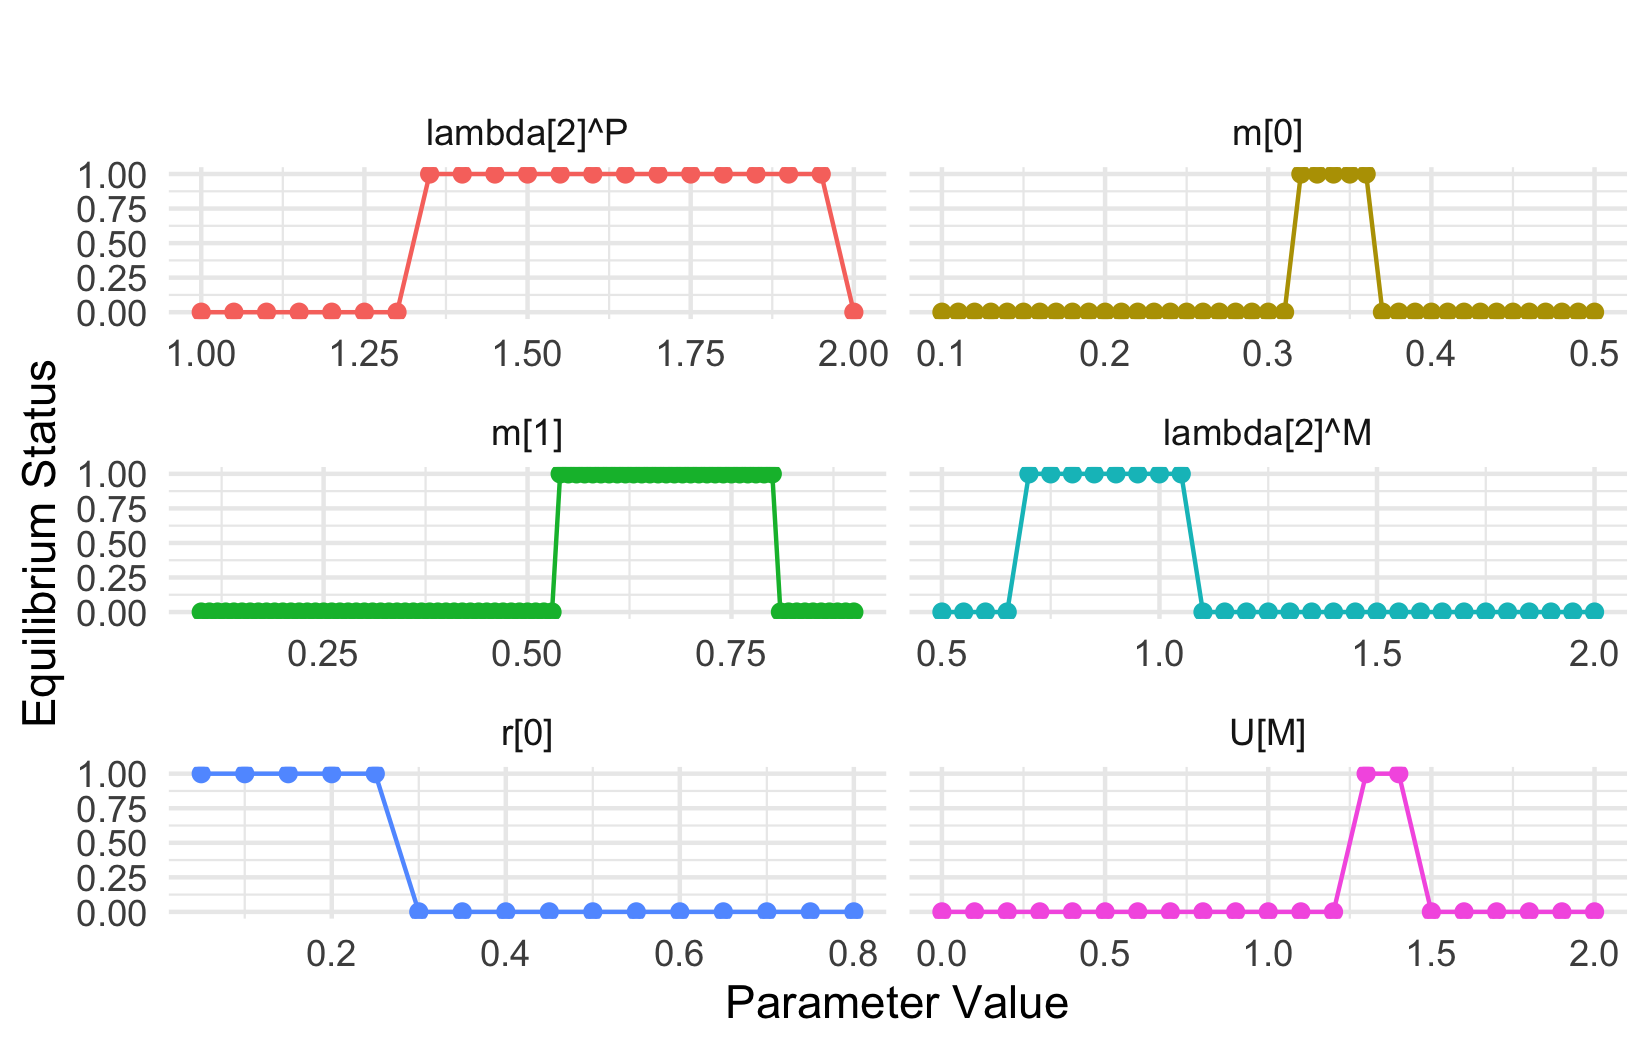
\includegraphics[keepaspectratio]{auten_formal_temp_files/figure-pdf/fig-statics-1.png}}

}

\caption{\label{fig-statics}Sensitivity of Equilibrium to Parameter
Changes}

\end{figure}%

Since a babbling equilibrium always exists
(\citeproc{ref-farrell1996CheapTalk}{Farrell and Rabin 1996}), we can
compare the results in the paper to any equilibrium outcome. In this
way, the babbling equilibrium stands as a ``baseline'' where the sources
of learning are just the outcomes of the battle. Note that \(P\) always
does at least as well under an influential equilibrium ex-ante as under
a babbling equilibrium. To see this, assume that the the game is such
that the probability that the state of the world is \(\omega_E = 1\) is
high. Assume that \(u_0\) is sufficiently high and passes the cutpoint
in Lemma~\ref{lem-pbelief1}. Moreover, assume that if \(P\) makes it to
round 2 \(\mu_2(s_1, r)\), will be above the cutpoint defined in
Equation~\ref{eq-cutpoint2}. Even if an equilibrium is a babbling
equilibrium, \(P\) will continue to escalate because of the high prior
probabilities.

To see that \(P\) is at least as well off, assume that an equilibrium is
influential. Keeping all other assumptions above the same. In such an
equilibrium, even one of the ones where it only occurs in the second
round, \(P\) would escalate in round 1, and then in round 2, it would
learn the true state of the world. \(P\) would thus escalate again at
the final round, obtaining their highest payoff. Alternatively, if the
true state of the world was actually \(\omega_E = 0\), then \(P\) would
withdraw at the last round, thus doing better than they would in a
babbling equilibrium. Hence, in an influential equilibrium, \(P\) always
does at least as well as they would in a babbling equilibrium, even one,
when the equilibrium is babbling in round one and separating in round 2.
Hence, honest communication, even if only in the second round, always
benefits \(P\).

\section{Discussion}\label{discussion}

Recall that the Military does two things in war: it fights the war and
provides information on how the battle went. In this model, the
Military's messaging strategy does not have a single monotonic effect on
conflict. In some scenarios, an informative equilibrium is associated
with a longer war, and in others, with a shorter war. Suppose that the
state of the world is such that \(\omega_E = 0\) but that \(P\)'s prior
belief is high enough to result in prolonged conflict. In such a
scenario, an informative equilibrium is associated with a shorter war,
but clearly, it need not always be. Assume that instead,
\(\omega_E = 1\) and \(\mu_0\) are just below the cutpoint defined in
Lemma~\ref{lem-pbelief1}. In a babbling equilibrium, this results in a
shorter war. However, in an influential equilibrium, \(P\) may instead
be informed about the state of the world and choose to continue the war.
However, such a result could be due to the modeling technology employed
here. Note that if we added a third player and bargaining, as in
Slantchev
(\citeproc{ref-slantchevPrincipleConvergenceWartime2003}{2003}), then
informative equilibrium would be associated with bargaining. If such a
signal led to complete information bargaining, the game would likely end
in peace (\citeproc{ref-fearonRationalistExplanationsWar1995}{Fearon
1995}). Influential equilibrium would likely be associated with shorter
wars under such scenarios.

However, the strict conditions needed to ensure this equilibrium mean
sthis equilibrium is hard to satisfy. As seen Figure~\ref{fig-statics},
even the equilibrium with partial communication is relatively sensitive.
For fully honest communication, nearly every exogenous parameter is
bounded between two values for \(M\) and \(P\). As such, the existence
of this equilibrium is unlikely to hold unless under narrow conditions.
Conversely, Proposition~\ref{prp-transition1} holds under a range, even
if it is a narrow range, of parameters and is thus more likely to come
up. This is largely due to the different boundary conditions needed for
Proposition~\ref{prp-transition1} since strictly increasing some
parameters helps obtain this equilibrium.

Substantively, we can treat this as follows: Early in a war, information
from the Military will likely be thrown out. It is unlikely that both
the Politician and the Military will have the same preferences over
outcomes early in the conflict because escalating a conflict in this
model funnels away resources from ``butter'' or other projects
(\citeproc{ref-powell1999shadow}{Powell 1999}) and funds the Military.
Of course, funding the Military is how you arm and train personnel and,
therefore, how you win a war, but the very act of funding the Military
may change preferences over outcomes. Earlier in the battle, and if the
transfer of resources is large and the costs of the war relatively low,
the Military obtains more resources; but as the war goes on, and the
transfer of future resources takes on a specific bound, then war may
incentivize honest communication. However, equilibria like
Proposition~\ref{prp-transition1} are sensitive to changes in
parameters. This may imply that honest communication between the
Military and the Politician is unlikely to happen early in the war and
is only likely to happen to the degree that continued war allows the
Military to have diverging preferences over outcomes.

\section{Conclusion}\label{conclusion}

In this model, I have attempted to explain under what conditions the
Military and Politican can have honest communication about a war effort
and to see how that impacts war duration. I have found that there are
narrow conditions under which the Military can provide credible
information during a war and that when these situations occur, it is
likely to come after more escalation. Moreover, the power shift at the
start of the game is key to this model. While something that impacts
power in the middle of a conflict may seem counterintuitive, there are
plenty of examples of such a scenario throughout history. We may think
of mass illness during war or perhaps wartime aid and funding as some
examples. One historical example comes from the French Invasion of
Russia of 1812. During the French Invasion of Russia in 1812, on the
long march to Moscow, the French army began to lose soldiers, not to the
cold but to disease
(\citeproc{ref-mikaberidzeLimitsOperationalArt2016}{Mikaberidze 2016};
\citeproc{ref-taltyIllustriousDeadTerrifying2009a}{Talty 2009}). While
Napoleon toured his camps and asked how many men were healthy and ready
to fight, his soldiers constantly inflated the numbers of soldiers that
were healthy in the grand armee
(\citeproc{ref-mikaberidzeLimitsOperationalArt2016}{Mikaberidze 2016});
hence, the political leaders at the time could not account for the full
strength of their army due to incentives for parts of the Military to
misrepresent the truth. In this illustrative example, Napoleon's
soldiers possess private information that the leader does not possess.
The leader would be better off with that information, but the signal was
effectively ignored because of the soldiers' incentives always to report
that they were doing well. Following his prior belief and having started
with around 700,000 soldiers
(\citeproc{ref-jankauskas2012IncideruntItaqueFossam}{Jankauskas 2012}),
Napoleon believed he was highly likely to win. The signals of his
soldiers and men were treated as babbling as they all said primarily
things Napoleon wanted to hear
(\citeproc{ref-gompert2014NapoleonsInvasionRussia}{Gompert, Binnendijk,
and Lin 2014}).

While we cannot know the counterfactual of how long the war would
continue had political leaders known the full extent of the losses, the
fact that it took until after Moscow was conquered for Napoleon to make
a hectic retreat is suggestive
(\citeproc{ref-gompert2014NapoleonsInvasionRussia}{Gompert, Binnendijk,
and Lin 2014}). Those who do the fighting, the dying, and presumably the
learning must report these changes to those who make decisions. Without
such reports, political leaders may learn more slowly from events than
they otherwise could. Another potential source of exogenous asymmetric
information, all but on the costs side, involves leader turnover. New
leaders who come into office shortly before or during a conflict have
different levels of resolve and may be more likely to prolong a
conflict. One potential statistical test of my argument would involve
leader transitions for a particular dyad with a conflict.

Another empirical implication is that leaders would seem to be more
likely to listen to the Military as the war progresses. Early on, when
the Military is eager to extract resources, it is unlikely that the
Politician will treat the Military as anything other than a babbling
equilibrium. However, the cost of war and the more minimal transfer of
resources may open up avenues of communication.

\newpage

\section{References}\label{references}

\phantomsection\label{refs}
\begin{CSLReferences}{1}{0}
\bibitem[\citeproctext]{ref-acemogluCyclesConflictEconomic2014}
Acemoglu, Daron, and Alexander Wolitzky. 2014. {``Cycles of {Conflict}:
{An Economic Model}.''} \emph{American Economic Review} 104 (4):
1350--67. \url{https://doi.org/10.1257/aer.104.4.1350}.

\bibitem[\citeproctext]{ref-baligaBargainingWarReview2019}
Baliga, Sandeep, and T. Sjöström. 2019. {``Bargaining and {War}: {A
Review} of {Some Formal Models}.''} \emph{Korean Economic Review} 29
(2): 235--66.

\bibitem[\citeproctext]{ref-downs1994ConflictAgencyGambling}
Downs, George W., and David M. Rocke. 1994. {``Conflict, {Agency}, and
{Gambling} for {Resurrection}: {The Principal-Agent Problem Goes} to
{War}.''} \emph{American Journal of Political Science} 38 (2): 362--80.
\url{https://doi.org/10.2307/2111408}.

\bibitem[\citeproctext]{ref-farrell1996CheapTalk}
Farrell, Joseph, and Matthew Rabin. 1996. {``Cheap {Talk}.''}
\emph{Journal of Economic Perspectives} 10 (3): 103--18.
\url{https://doi.org/10.1257/jep.10.3.103}.

\bibitem[\citeproctext]{ref-fearonRationalistExplanationsWar1995}
Fearon, James. 1995. {``Rationalist {Explanations} for {War}.''}
\emph{International Organization} 49 (3): 379--414.
\url{https://www.jstor.org/stable/2706903}.

\bibitem[\citeproctext]{ref-fey2010WhenShuttleDiplomacy}
Fey, Mark, and Kristopher W. Ramsay. 2010. {``When Is Shuttle Diplomacy
Worth the Commute? {Information Sharing} Through {Mediation}.''}
\emph{World Politics} 62 (4): 529--60.
\url{https://www.jstor.org/stable/40891389}.

\bibitem[\citeproctext]{ref-filsonBargainingModelWar2002}
Filson, Darren, and Suzanne Werner. 2002. {``A {Bargaining Model} of
{War} and {Peace}: {Anticipating} the {Onset}, {Duration}, and {Outcome}
of {War}.''} \emph{American Journal of Political Science} 46 (4):
819--37. \url{https://doi.org/10.2307/3088436}.

\bibitem[\citeproctext]{ref-filsonBargainingFightingImpact2004}
---------. 2004. {``Bargaining and {Fighting}: {The Impact} of {Regime
Type} on {War Onset}, {Duration}, and {Outcomes}.''} \emph{American
Journal of Political Science} 48 (2): 296--313.
\url{https://doi.org/10.1111/j.0092-5853.2004.00071.x}.

\bibitem[\citeproctext]{ref-filsonDynamicsBargainingWar2007}
---------. 2007a. {``The {Dynamics} of {Bargaining} and {War}.''}
\emph{International Interactions} 33 (1): 31--50.
\url{https://doi.org/10.1080/03050620601155656}.

\bibitem[\citeproctext]{ref-filsonSensitivityCostsFighting2007}
---------. 2007b. {``Sensitivity to {Costs} of {Fighting} Versus
{Sensitivity} to {Losing} the {Conflict}: {Implications} for {War
Onset}, {Duration}, and {Outcomes}.''} \emph{Journal of Conflict
Resolution} 51 (5): 691--714.
\url{https://doi.org/10.1177/0022002707304426}.

\bibitem[\citeproctext]{ref-gompert2014NapoleonsInvasionRussia}
Gompert, David C., Hans Binnendijk, and Bonny Lin. 2014. {``Napoleon's
{Invasion} of {Russia}, 1812.''} In \emph{Blinders, {Blunders}, and
{Wars}}, 41--52. What {America} and {China Can Learn}. RAND Corporation.
\url{https://www.jstor.org/stable/10.7249/j.ctt1287m9t.10}.

\bibitem[\citeproctext]{ref-heifetzEscalationDelayProtracted2005}
Heifetz, Aviad, and Ella Segev. 2005. {``Escalation and Delay in
Protracted International Conflicts.''} \emph{Mathematical Social
Sciences} 49 (1): 17--37.
\url{https://doi.org/10.1016/j.mathsocsci.2004.08.001}.

\bibitem[\citeproctext]{ref-jankauskas2012IncideruntItaqueFossam}
Jankauskas, Rimantas. 2012. {``Inciderunt Itaque in Fossam Quam Sibi
Ipsi Fecerunt: {MASS GRAVE OF NAPOLEON}'{S SOLDIERS IN VILNIUS DECEMBER}
1812.''} \emph{Revue Des Études Slaves} 83 (4): 981--91.
\url{https://www.jstor.org/stable/43272231}.

\bibitem[\citeproctext]{ref-kraininRationalQuagmiresAttrition2020}
Krainin, Colin, Caroline Thomas, and Thomas Wiseman. 2020. {``Rational
{Quagmires}: {Attrition}, {Learning}, and {War}.''} \emph{Quarterly
Journal of Political Science} 15 (3): 369--400.
\url{https://doi.org/10.1561/100.00018008}.

\bibitem[\citeproctext]{ref-mikaberidzeLimitsOperationalArt2016}
Mikaberidze, Alexander. 2016. {``The {Limits} of the {Operational Art}:
{Russia} 1812.''} In \emph{Napoleon and the Operational Art of War :
Essays in Honor of {Donald D}. {Horward}}. History of {Warfare},
{Volume} 110. Leiden, Netherlands: Brill.

\bibitem[\citeproctext]{ref-powell1999shadow}
Powell, Robert. 1999. \emph{In the Shadow of Power: {States} and
Strategies in International Politics}. Princeton University Press.

\bibitem[\citeproctext]{ref-powellBargainingLearningFighting2004}
---------. 2004. {``Bargaining and {Learning While Fighting}.''}
\emph{American Journal of Political Science} 48 (2): 344--61.
\url{https://doi.org/10.1111/j.0092-5853.2004.00074.x}.

\bibitem[\citeproctext]{ref-powellPersistentFightingShifting2012}
---------. 2012. {``Persistent {Fighting} and {Shifting Power}.''}
\emph{American Journal of Political Science} 56 (3): 620--37.
\url{https://doi.org/10.1111/j.1540-5907.2011.00575.x}.

\bibitem[\citeproctext]{ref-sanaeiTimeEssenceCausal2019}
Sanaei, Ali. 2019. {``Time Is of the Essence: {The} Causal Effect of
Duration on Support for War.''} \emph{Journal of Peace Research} 56 (6):
783--96. \url{https://doi.org/10.1177/0022343319834984}.

\bibitem[\citeproctext]{ref-shirkeyUncertaintyWarDuration2016}
Shirkey, Zachary C. 2016. {``Uncertainty and {War Duration}.''}
\emph{International Studies Review} 18 (2): 244--67.
\url{https://doi.org/10.1093/isr/viv005}.

\bibitem[\citeproctext]{ref-slantchevPrincipleConvergenceWartime2003}
Slantchev, Branislav L. 2003. {``The {Principle} of {Convergence} in
{Wartime Negotiations}.''} \emph{American Political Science Review} 97
(4): 621--32. \url{https://doi.org/10.1017/S0003055403000911}.

\bibitem[\citeproctext]{ref-smithBargainingNatureWar2004}
Smith, Alastair, and Allan C. Stam. 2004. {``Bargaining and the {Nature}
of {War}.''} \emph{Journal of Conflict Resolution} 48 (6): 783--813.
\url{https://doi.org/10.1177/0022002704268026}.

\bibitem[\citeproctext]{ref-smithMilitaryCoalitionsPolitics2021}
Smith, Bradley C. 2021. {``Military {Coalitions} and the {Politics} of
{Information}.''} \emph{The Journal of Politics} 83 (4): 1369--82.
\url{https://doi.org/10.1086/711625}.

\bibitem[\citeproctext]{ref-smithMilitarizedDisputesUncertainty2019}
Smith, Bradley C., and William Spaniel. 2019. {``Militarized {Disputes},
{Uncertainty}, and {Leader Tenure}.''} \emph{Journal of Conflict
Resolution} 63 (5): 1222--52.
\url{https://doi.org/10.1177/0022002718789738}.

\bibitem[\citeproctext]{ref-spanielSlowLearnBargaining2016}
Spaniel, William, and Peter Bils. 2016. {``Slow to {Learn}:
{Bargaining}, {Uncertainty}, and the {Calculus} of {Conquest}.''}
\emph{Journal of Conflict Resolution} 62 (4): 774--96.
\url{https://doi.org/10.1177/0022002716662688}.

\bibitem[\citeproctext]{ref-taltyIllustriousDeadTerrifying2009a}
Talty, Stephan. 2009. \emph{The Illustrious Dead : The Terrifying Story
of How Typhus Killed {Napoleon}'s Greatest Army / {Stephan Talty}.} 1st
ed. New York: Crown Publishers.

\bibitem[\citeproctext]{ref-wagnerBargainingWar2000}
Wagner, R. Harrison. 2000. {``Bargaining and {War}.''} \emph{American
Journal of Political Science} 44 (3): 469--84.
\url{https://doi.org/10.2307/2669259}.

\bibitem[\citeproctext]{ref-wuLeadersStatesReputations2018}
Wu, Cathy Xuanxuan, and Scott Wolford. 2018. {``Leaders, {States}, and
{Reputations}.''} \emph{Journal of Conflict Resolution} 62 (10):
2087--117. \url{https://doi.org/10.1177/0022002718786001}.

\bibitem[\citeproctext]{ref-yaredDynamicTheoryWar2010}
Yared, Pierre. 2010. {``A Dynamic Theory of War and Peace.''}
\emph{Journal of Economic Theory} 145 (5): 1921--50.
\url{https://doi.org/10.1016/j.jet.2010.04.005}.

\end{CSLReferences}

\newpage

\section{Appendix}\label{sec-appendix}

% Include the appendix TOC at the very top of the appendix
% Mark the start of the appendix for TOC isolation
\startcontents[appendix]
% Include the appendix TOC at the very top of the appendix
\renewcommand{\contentsname}{Appendix Contents}  % Title for the appendix TOC
\setcounter{tocdepth}{3}  % Adjust the depth of TOC entries (e.g., include subsections)
\begin{center}
\textbf{Appendix Contents}
\end{center}
\startcontents[appendix]  % Begin a TOC for the appendix
\printcontents[appendix]{}{-1}{\setcounter{tocdepth}{3}}  % Print TOC for appendix

\subsection{Table}\label{table}

\begin{longtable}[]{@{}ll@{}}
\caption{Table of Notation Used}\label{tbl-symbols}\tabularnewline
\toprule\noalign{}
Symbol & Meaning \\
\midrule\noalign{}
\endfirsthead
\toprule\noalign{}
Symbol & Meaning \\
\midrule\noalign{}
\endhead
\bottomrule\noalign{}
\endlastfoot
\(P\) & Politician \\
\(M\) & Military \\
\(\omega_E\) & state of the world, \\
\(q(\omega_E)\) & Enemy's probability of winning \\
\(m(\omega_E)\) & Probability that \(P\) and \(M\) win \\
\(r(\omega_E)\) & Probability of stalemate \\
\(s_t\) & Signal chosen by \(M\) indexed by period \\
\(a_t\) & Action chosen by \(P\) indexed by period \\
\(\lambda_{P}^t\) & Reservation value for \(P\) \\
\(\lambda_{M}t\) & Reservation value for \(M\) \\
\(U_i\) & Payoff for player \(i\) when winning \\
\(V_i(\mu)\) & Flow payoff \\
\(\mu_t()\) & Beliefs of \(P\) \\
\(\delta\) & Discount factor \\
\(x_i\) & Stage payoff \\
\end{longtable}

\subsection{Proofs}\label{proofs}

\subsubsection{\texorpdfstring{Proof of
Lemma~\ref{lem-4}}{Proof of Lemma~}}\label{proof-of-lem-4}

\begin{proof}
Let us find a threshold for the belief that the state of the world is
\(\omega_E = 1\) given some strategy by \(M\). Again, assume that
Equation~\ref{eq-assump_p_r2} holds, then the following expresses the
threshold for the belief for \(P\) that they will escalate:

\[
\begin{aligned}
\mu_2(r, s_2) \cdot m(1)' \cdot U_P' + (1 - \mu_2(r, s_2)) \cdot m(0)' \cdot U_P' > \lambda^2_P \\
\mu_2(r, s_2) [m(1)' U_P' - m(0)' U_P'] +  m(0)' \cdot U_P' > \lambda^2_P\\
\end{aligned}
\]

\begin{equation}\phantomsection\label{eq-cutpoint_r2}{
\mu_2(r, s_2) > \frac{\lambda^2_P -  m(0)' \cdot U_P'}{m(1)' U_P' - m(0)' U_P'}
}\end{equation}

Given Equation~\ref{eq-assump_p_r2}, then \(P\) must play as follows in
round 2

\[
\sigma_P^{2*} = 
\begin{cases} 
a_2 = e & \text{if } \mu_2(r, s_2) > \frac{\lambda^2_P - m(0)' U_P '}{m(1)' U_P' - m(0)' U_P'}\\
a_2 = w & \text{if } \mu_2(r, s_2) < \frac{\lambda^2_P - m(0)' U_P '}{m(1)' U_P' - m(0)' U_P'}
\end{cases}
\]
\end{proof}

\subsubsection{\texorpdfstring{Proof of
Proposition~\ref{prp-unalign2}}{Proof of Proposition~}}\label{proof-of-prp-unalign2}

If Equation~\ref{eq-mpref_r2} fails, then the only equilibrium in the
second round is a babbling equilibrium, which is as follows:

\[
\sigma_P^{2*} = 
\begin{cases} 
a_2 = e & \text{if } \mu_2(s_1, r) > \frac{\lambda^2_P - m(0)' U_P '}{m(1)' U_P' - m(0)' U_P'}\\
a_2 = w & \text{if } \mu_2(s_1, r) < \frac{\lambda^2_P - m(0)' U_P '}{m(1)' U_P' - m(0)' U_P'}
\end{cases}
\]

\begin{itemize}
\tightlist
\item
  \(P's\) updated belief is the prior belief, which is equal to the
  following:
\end{itemize}

\[
\begin{aligned}
\mu_2(s_1, s_2) =  \mu_2(r, s_2)\\
\mu_2(r, s_2) =  \frac{r(1) \cdot p}{r(1) \cdot p + (1 - p) \cdot r(0)}
\end{aligned}
\]

\begin{itemize}
\tightlist
\item
  Any strategy by \(M\) is in equilbrium where \(\sigma_P^{2*}\) is a
  probability distribution over the signals
\end{itemize}

\[
\sigma_M^{2*} \in [0, 1]
\]

Hence, a PBE consists of the following three objects

\([\sigma_P^{2*}, \sigma_M^{2*},  \mu_2(r, s_2])\)

\begin{proof}
Since Equation~\ref{eq-mpref_r2} fails, and as shown in
Lemma~\ref{lem-nec_cond}, we know that this equilibrium will be a
babbling equilibrium. Because we assume that
Equation~\ref{eq-assump_p_r2} holds, \(P\) prefers to escalate when
facing the weak type and withdraw when facing the strong type.
Lemma~\ref{lem-4} gives us the cutoff for what \(P\) has to believe to
escalate. As such, all that is left is to define the beliefs and how
they are updated.

First, let us define \(\mu_2(s_1, r)\). Such a belief is defined as
follows:

\[
\begin{aligned}
\mu_2(s_1, r) = \frac{Pr(\text{stalemate}|\omega_E=1)}{Pr(\text{stalemate})}\\
= \frac{r(1) p}{r(1)p + (1 - p) r(0)} 
\end{aligned}
\]

The posterior belief after \(M\) sends a signal in the final round is
defined as follows:

\[
\mu_2(r, s_2) = \frac{\mu_2(s_1, r) \cdot \sigma_M^2(s_2 = e|\omega=1)}{\mu_2(s_1, r) \cdot \sigma_M^2(s_2 = e|\omega=1) + [1 - \mu_2(s_1, r)] \cdot \sigma_M^2(s_2 = e|\omega=0)}
\]

However, according to Lemma~\ref{lem-5}, no updating can occur since
\(M\)'s signal is ignored. Hence \(\mu_2(r, s_2) = \mu_2(s_1, r)\).This
means that \(P\)'s action is entirely determined by \(\mu_2(r, s_2)\) as
shown in Lemma~\ref{lem-4}. Moreover, there are no strong conditions or
boundaries to put on this equilibrium so long as
Equation~\ref{eq-assump_p_r2} holds, then this babbling equilibrium
always exists (\citeproc{ref-farrell1996CheapTalk}{Farrell and Rabin
1996}) since the only necessary condition is \(P\)'s preferences.
Putting it all together, the following is the equilibrium assessment:

\[
\sigma_P^{2*} = 
\begin{cases} 
a_2 = e & \text{if } \mu_2(s_1, r) > \frac{\lambda^2_P - m(0)' U_P '}{m(1)' U_P' - m(0)' U_P'}\\
a_2 = w & \text{if } \mu_2(s_1, r) < \frac{\lambda^2_P - m(0)' U_P '}{m(1)' U_P' - m(0)' U_P'}
\end{cases}
\]

\[
\begin{aligned}
\mu_2(r, s_2) =  \mu_2(s_1, r)\\
\mu_2(s_1, r) =  \frac{r(1) \cdot p}{r(1) \cdot p + (1 - p) \cdot r(0)}
\end{aligned}
\] \[
\sigma_M^{2*} \in [0, 1]
\]
\end{proof}

\subsubsection{\texorpdfstring{Proof of
Proposition~\ref{prp-aligned2}}{Proof of Proposition~}}\label{proof-of-prp-aligned2}

If Equation~\ref{eq-mpref_r2} holds in round 2, then there exists an
influential equilibrium that is characterized by the following
assessment:

\[
\sigma_P^{2*} = 
\begin{cases} 
a_2 = e & \text{if } \mu_2(s_1, r) > \frac{\lambda^2_P - m(0)' U_P '}{m(1)' U_P' - m(0)' U_P'}\\
a_2 = w & \text{if } \mu_2(s_1, r) < \frac{\lambda^2_P - m(0)' U_P '}{m(1)' U_P' - m(0)' U_P'}
\end{cases}
\]

\[
\mu_2(r, s_2) =
\begin{cases} 
 = 1 & \text{if } \quad s_2 = e \\
= 0 & \text{if } \quad s_2 = w  \\
\end{cases}
\]

\[
\sigma_M^{2*} = 
\begin{cases} 
s_2 =  e & \text{if } \quad \omega_E = 1 \\
s_2 =  w & \text{if } \quad \omega_E = 0 \\
\end{cases}
\]

\begin{proof}
Recall the necessary conditions needed for an influential equilibrium.
The first condition is met in the second round based on
Equation~\ref{eq-mpref_r2}. The proof thus needs to show that \(P\)
learns \(M\) and that these signals change \(P\)'s behavior in order for
an equilibrium to be influential.

Since, Equation~\ref{eq-mpref_r2} holds, if the equilbirum is
influential then \(M\) must have the following optimal strategy:

\[
\sigma_M^{2*} = 
\begin{cases} 
s_2 =  e & \text{if } \quad \omega_E=1 \\
s_2 = w & \text{if} \quad \omega_E= 0\\
\end{cases}
\]

Next, we see if, in turn, \(P\) updates their beliefs. Suppose the state
of the world is \(\omega_E = 1\).

\[
\begin{aligned}
\mu_2(r, s_2) = \frac{\mu_(s_1, r) \cdot 1}{\mu(w|S) \cdot 1 + (1 - \mu_(s_1, r) \cdot 0}\\
= 1
\end{aligned}
\]

Suppose instead that the state of the world is instead \(\omega_E = 1\),
then \(P\) updates their belief as follows:

\[
\begin{aligned}
\mu_2(r, s_2) = \frac{\mu_(s_1, r) \cdot 0}{\mu_(s_1, r)\cdot 0 + (1 - \mu_(s_1, r)) \cdot 0}\\
\end{aligned}
\]

Clearly, you cannot divide by zero. As such, we cannot use Bayes rule
here. I thus set the belief to \(0\) since if we were to define the
mirror belief of \(\mu_2(r, s_2)\) as to whether a strong type exists,
it would be \(1\).

Since \(P\)'s belief changes based on the signal, we have the second
part of the necessary condition. Lastly, we simply need to check how
\(P\)'s actions change. Since the decision rule outlined in
Lemma~\ref{lem-4} still holds, and we are still assuming
Equation~\ref{eq-assump_p_r2}, the following is an equilibrium strategy:
\[
\sigma_P^{2*} = 
\begin{cases} 
a_2 = e & \text{if } \mu_2(s_1, r) > \frac{\lambda^2_P - m(0)' U_P '}{m(1)' U_P' - m(0)' U_P'}\\
a_2 = w & \text{if } \mu_2(s_1, r) < \frac{\lambda^2_P - m(0)' U_P '}{m(1)' U_P' - m(0)' U_P'}
\end{cases}
\]

This equilibrium is a special case where the belief equals \(1\) or
\(0\). Thus, we have the third part of the necessary condition, and
\(P\)'s actions change based upon \(M\)'s signal, and \(P\) escalates
when \(\omega_E=1\) and withdraws when \(\omega_E=0\).

A number of conditions need to hold for an influential separating
equilibrium to be possible, but I will address these in
Proposition~\ref{prp-aligned1}.
\end{proof}

\subsubsection{\texorpdfstring{Proof of
Lemma~\ref{lem-pbelief1}}{Proof of Lemma~}}\label{proof-of-lem-pbelief1}

\emph{If Equation~\ref{eq-assump_p_r1} holds, then} \(P\)'s optimal
strategy in round 1 can be specified with reference to the round 1
belief and is thus defined as follows:

\[
\sigma^{1*}_P = 
\begin{cases}
a_1= e  & \text{if } \quad\mu(s_1)
> \frac{\lambda^1_P - m(0)U_P - r(0)(x_P + \delta V_P(\mu_2))}
 {U_P[ m(1) - m(0) ]+ x_P [r(1) -r(0)] 
 + \delta (r(1)V_P'(\mu_2) - r(0)V_P(\mu_2))}\\
a_1 = w  & \text{if } \mu(s_1)
< \frac{\lambda^1_P - m(0)U_P - r(0)(x_p + \delta V_P(\mu_2))}
 {U_P[ m(1) - m(0) ]+ x_P [r(1) -r(0)] 
 + \delta (r(1)V_P'(\mu_2) - r(0)V_P(\mu_2))}
\end{cases}
\]

\begin{proof}
The belief is obtained by construction, while the cut point is found by
how confident \(P\) has to be in the weak type relative to their
expected payoffs for the game.

\[
\mu(s_1) = \frac{p \cdot \sigma^1_M}{p \cdot \sigma^1_M + (1 - p) \cdot \sigma^1_m(e|t = s)}
\]

The cut point is defined as follows:

\begin{equation}\phantomsection\label{eq-beliefr1}{
\begin{aligned}
&\mu(s_1) m(1) U_P
+ \mu(s_1)[r(0)(\delta V_P(\mu_2)' + x_P)] \\
&+ (1 - \mu(s_1)) m(0) U_P 
+ (1 - \mu(s_1) [m(0) x_P + \delta V_P(\mu_2)] > \lambda^1_P, \\
&\mu(s_1)[U_P (m(1)- m(0)) 
+ x_P(r(1) - r(0)) 
+ \delta (r(1)V_P'(\mu_2) - r(0)V_P(\mu_2))] \\
&\quad > \lambda^1_P - m(0)U_P 
+ r(0) x_P + \delta V_P(\mu_2), \\
& \mu(s_1)
> \frac{\lambda^1_P - m(0)U_P - r(0)(x_P + \delta V_P(\mu_2))}
 {U_P[ m(1) - m(0) ]+ x_P [r(1) -r(0)] 
 + \delta (r(1)V_P'(\mu_2) - r(0)V_P(\mu_2))}
\end{aligned}
}\end{equation}

This, in turn determines \(P\)'s optimal strategy in round 1

\begin{equation}\phantomsection\label{eq-stratp}{
\sigma^{1*}_P = 
\begin{cases}
a_1= e  & \text{if } \quad\mu(s_1)
> \frac{\lambda^1_P - m(0)U_P - r(0)(x_P + \delta V_P(\mu_2))}
 {U_P[ m(1) - m(0) ]+ x_P [r(1) -r(0)] 
 + \delta (r(1)V_P(\mu_2)' - r(0)V_P(\mu_2))}\\
a_1 = w  & \text{if } \mu(s_1)
< \frac{\lambda^1_P - m(0)U_P - r(0)(x_P + \delta V_P(\mu_2))}
 {U_P[ m(1) - m(0) ]+ x_P [r(1) -r(0)] 
 + \delta (r(1)V_P'(\mu_2) - r(0)V_(\mu_2)P)}
\end{cases}
}\end{equation}
\end{proof}

\subsubsection{\texorpdfstring{Proof of
Proposition~\ref{prp-unaligned1}}{Proof of Proposition~}}\label{proof-of-prp-unaligned1}

If Equation~\ref{eq-mpref_r1} and Equation~\ref{eq-mpref_r2} fail and
Equation~\ref{eq-assump_p_r1} holds, then there must be a babbling
equilibrium that consists of the following elements:

\[
\sigma^{*}_P = 
\begin{cases}
a_1= e  & \text{if } \quad\mu(s_1)
> \frac{\lambda^1_P - m(0)U_P - r(0)(x_P + \delta V_P(\mu_2))}
 {U_P[ m(1) - m(0) ]+ x_P [r(1) -r(0)] 
 + \delta (r(1)V_P'(\mu_2) - r(0)V_P(\mu_2)}\\
a_1 = w  & \text{if } \mu(s_1)
< \frac{\lambda^1_P - m(0)U_P - r(0)(x_p + \delta V_P(\mu_2))}
 {U_P[ m(1) - m(0) ]+ x_P [r(1) -r(0)] 
 + \delta (r(1)V_P'(\mu_2) - r(0)V_P(\mu_2))}\\
a_2 = e & \text{if } \mu_2(s_1, r) > \frac{\lambda^2_P - m(0)' U_P '}{m(1)' U_P' - m(0)' U_P'}\\
a_2 = w & \text{if } \mu_2(s_1, r) < \frac{\lambda^2_P - m(0)' U_P '}{m(1)' U_P' - m(0)' U_P'}\\
\end{cases}
\]

Any signal or mixture of signals is in equilibrium for \(M\):

\[
\sigma^{*}_M \in [0, 1]
\]

Moreover, \(P\)'s belief always equals the prior belief.

\[
\mu^*= 
\begin{cases}
p  & \text{in } \quad \text{round 1}\\
\mu_2(s_1, r)  & \text{in } \quad \text{round 2}\\
\end{cases}
\]

\begin{proof}
The proof is primarily a matter of combining previous lemmas and
propositions. \(P\)'s optimal strategy and beliefs for round two are
proved in Proposition~\ref{prp-unalign2}, and their optimal strategy and
beliefs for round 1 are proved in Lemma~\ref{lem-pbelief1}. Similarly,
the fact that \(M\) can play any strategy comes from Lemma~\ref{lem-5}.

Because \(M\)'s signal is always treated as noise and ignored, \(M\)
sends any signal. Because we have assumed that
Equation~\ref{eq-assump_p_r1} holds, \(P\)'s optimal beliefs are simple.
If their belief is above the threshold Equation~\ref{eq-beliefr1} then
they escalate, and if their belief is below the threshold
Equation~\ref{eq-beliefr1} they withdraw. If a stalemate occurs, then
\(P\) revises their belief. Again, if their belief is above the
threshold defined in Proposition~\ref{prp-unalign2}, they escalate, and
if it is below that cutpoint, they withdraw. Prior probabilities and the
general cutpoints in the model entirely determine \(P\)'s welfare.
\end{proof}

\subsubsection{\texorpdfstring{Proof of
Proposition~\ref{prp-aligned1}}{Proof of Proposition~}}\label{proof-of-prp-aligned1}

If Equation~\ref{eq-assump_p_r1}, Equation~\ref{eq-mpref_r1}, and the
number of specifications specified below all hold, then an influential
equilibrium exists where separating occurs and is of the following
character:

\[
\sigma^{*}_M = 
\begin{cases}
s = e  & \text{if } \quad \omega_E = 1\\
s = w  & \text{if } \quad \omega_E = 0 \\
\end{cases}
\]

\[
\sigma^{*}_P = 
\begin{cases}
a_1= e  & \text{if } \quad\mu(s_1)
> \frac{\lambda^1_P - m(0)U_P - r(0)(x_P + \delta V_P(\mu_2))}
 {U_P[ m(1) - m(0) ]+ x_P [r(1) -r(0)] 
 + \delta (r(1)V_P'(\mu_2) - r(0)V_P(\mu_2)}\\
a_1 = w  & \text{if } \mu(s_1)
< \frac{\lambda^1_P - m(0)U_P - r(0)(x_p + \delta V_P(\mu_2))}
 {U_P[ m(1) - m(0) ]+ x_P [r(1) -r(0)] 
 + \delta (r(1)V_P'(\mu_2) - r(0)V_P(\mu_2))}\\
a_2 = e & \text{if } \mu_2(s_1, r) > \frac{\lambda^2_P - m(0)' U_P '}{m(1)' U_P' - m(0)' U_P'}\\
a_2 = w & \text{if } \mu_2(s_1, r) < \frac{\lambda^2_P - m(0)' U_P '}{m(1)' U_P' - m(0)' U_P'}\\
\end{cases}
\]

\[
\mu^* = 
\begin{cases}
\mu_1(s_1) = 1 & \text{ if} \quad t = w\\
\mu(t= s| \sigma^{*}_m) = 1 & \text{ if} \quad t = s
\end{cases}
\]

\begin{proof}
If \(M\) fully separates in round 1, then \(P\) knows with certainty the
type of enemy they are facing. Hence, Equation~\ref{eq-mpref_r2} becomes
irrelevant to this equilibrium. All that matters is \(M\)'s preferences
over outcomes in round 1. Two things must be true for \(M\) to fully
separate in the first period: First, Equation~\ref{eq-mpref_r1} must
hold

\[
m(1) + \frac{r(1)(\delta V_M'(\mu_2) + x_M)}{U_M} > \frac{\lambda^1_M}{U_M} > m(0) + \frac{r(0)(\delta V_M(\mu_2) + x_M)}{U_M}\\
\]

Second, Equation~\ref{eq-assump_p_r1} must hold for \(P\) to care at all
about separating signals:

\[
m(1) + \frac{r(1)'(\delta V_P'(\mu_2) + x_P)}{U_P} > \frac{\lambda^1_P}{U_P} > m(0) + \frac{r(0)'(\delta V_P(\mu_2) + x_P)}{U_p}\\
\]

Assume that such an equilibrium exists. If it does, then we know the
continuation payoffs are as follows:

\[
\begin{aligned}
V_P(\mu) = \lambda^2_P\\
V_P'(\mu)  = U_P' m(1)''\\
V_M(\mu)  = \lambda^2_M\\
V_M'(\mu)  = U_M' m(1)'' \\
\end{aligned}
\]

The first part of the proof is essentially a piecing together of
previous results. All of the round two results come from
Proposition~\ref{prp-aligned2}, such as optimal strategies for both
players and round 2 beliefs. \(P\)'s optimal strategies come from
Lemma~\ref{lem-pbelief1}, and \(M\)'s behavior comes from
Proposition~\ref{prp-aligned2} and Lemma~\ref{lem-nec_cond}. \(P\)'s
beliefs are always certain, as I demonstrate by construction. When the
enemy is weak, then \(P\) updates their beliefs as follows:

\[
\mu_1(s_1) = \frac{p \cdot \ 1}{p \cdot 1+ (1 - p) \cdot 0} = 1
\]

Moreover, because they know the enemy is weak in round 1, this
translates to round 2's beliefs:

\[
\mu_2(s_1, r) = \frac{r(1) \cdot \ 1}{r(1) \cdot 1+ r(0)\cdot 0} = 1
\]

The second part of the proof involves the manipulation of the utility
equations of \(M\) and \(P\) to see what values of exogenous variables
can sustain this equilibrium. Several parameters must fall in boundary
conditions. First, \(\delta\), the common discount factor must satisfy
many inequalities:

\[
\begin{aligned}
U_M m(1) + r(1)(\delta V_M'(\mu_2) + x_M) > \lambda^1_M\\
\delta > \frac{\lambda^1_M - U_M m(1) - r(1)x_M}{ U_M' m(1)'r(1)}
\end{aligned}
\]

and

\[
\begin{aligned}
U_M m(0) + r(0)(\delta V_M(\mu_2) + x_M) <\lambda^1_M\\
\delta < \frac{\lambda^1_M - U_M m(0) - r(0)x_M}{ \lambda^2_Mr(0)}
\end{aligned}
\]

This means the following must hold:

\begin{equation}\phantomsection\label{eq-delta_sep_m}{
\frac{\lambda^1_M - U_M m(1) - r(1)x_M}{ U_M' m(1)'r(1)}<\delta < \frac{\lambda^1_M- U_M m(0) - r(0)x_M}{ \lambda^2_M r(0)}
}\end{equation}

The mirror inequality results in the following inequality that
\(\delta\) must satisfy with respect to \(P\)

\begin{equation}\phantomsection\label{eq-delta_sep_p}{
\frac{\lambda^1_P - U_P m(1) - r(1)x_P}{ U_P' m(1)'r(1)}<\delta < \frac{\lambda^1_P - U_P m(0) - r(0)x_P}{ \lambda^2_P r(0)}
}\end{equation}

Next, let us find what \(P\)'s utility for victory must be to sustain
such an equilibrium. For \(P\), recall that their resources diminish
with each round. As such, we can rewrite the second round utility of
winning as follows: \(U_P' = U_P - \Delta U_P\). In turn, this allows us
to rewrite the inequality below:

\[
\begin{aligned}
U_P m(1) + r(1)(V_P(\mu_2)'\delta + x_P) > \lambda^1_P\\
U_P > \frac{\lambda^1_P - r(1)'[ \Delta U_P m(1)' \delta - x_P]}{m(1) + r(1)\delta m(1)'}
\end{aligned}
\]

A similar process for the other side of the inequality leaves us with
the following:

\begin{equation}\phantomsection\label{eq-win_sep_p}{
\begin{aligned}
\frac{ \lambda^1_P - r(0)[\lambda^2_P \delta + x_P]}{m(0)} > U_P > \frac{\lambda^1_P - r(1)'[ \Delta U_P m(1)' \delta + x_P]}{m(1) + r(1)\delta m(1)'}\\
\end{aligned}
}\end{equation}

Performing the same comparison for \(M\) while bearing in mind that
\(U_M' = U_M + \Delta U_M\) reveals the following inequality

\[
\frac{\lambda^1_M - r(0)[\delta \lambda^2_M + x_P]}{m(0)} > U_M > \frac{\lambda^1_M- r(1)[\Delta U_M \delta m(1)'  + x_P]}{m(1)}
\]

Lastly, stage payoffs need to be examined. \(x_M\) must take on the
following values:

\[
\begin{aligned}
U_M m(1) + r(1)(\delta V_M'(\mu_2) + x_M) > \lambda^1_M\\
x_M > \frac{\lambda^1_M-U_M m(1) - r(1)\delta U_M'm(1)' }{r(1)}
\end{aligned}
\]

Which amounts to the following inequality:

\begin{equation}\phantomsection\label{eq-stage_sep_m}{
\begin{aligned}
\frac{\lambda^1_M -U_M m(1) - r(1)\delta U_M'm(1)' }{r(1)}<x_M < \frac{\lambda^1_M-U_M m(0) - r(0)\delta\lambda^2_M}{r(0)}
\end{aligned}
}\end{equation}

A similar process reveals the following for \(P\)

\[
\begin{aligned}
U_P m(1) + r(1)(V_P'(\mu_2)\delta + x_P) > \lambda^1_P\\
x_P > \frac{\lambda^1_P - U_P m(1) - r(1)U_P' m(1)' \delta}{r(1)} \\
\end{aligned}
\]

Which entails the following:

\begin{equation}\phantomsection\label{eq-stage_sep_p}{
\begin{aligned}
\frac{\lambda^1_P - U_P m(0) - r(0) \lambda^2_P \delta}{r(0)} > x_P > \frac{\lambda^1_P - U_P m(1) - r(1)U_P' m(1)' \delta}{r(1)}\\
\end{aligned}
}\end{equation}

For both players, the following being either strictly higher or lower
helps sustain the equilibrium: \[
\begin{aligned}
U_i m(1) + r(1)[ \delta V_i'(\mu_2) + x_i] > \lambda^1_i\\
m(1) > \frac{\lambda^1_i -r(1)[\delta V_i'(\mu_2) + x_i ]}{U_i}
\end{aligned}
\]

\[
\begin{aligned}
U_i m(1) + r(1)[ \delta V_i'(\mu_2) + x_i] > \lambda^1_i\\
r(1) > \frac{\lambda^1_i - U_i m(1)}{[\delta V_i'(\mu_2) + x_i ]}
\end{aligned}
\]

The mirror expression that needs to be as small as possible is as
follows:

\[
\begin{aligned}
m(0) < \frac{\lambda^1_i -r(0)[\delta V_i(\mu_2) + x_i ]}{U_i}
\end{aligned}
\]

and

\[
\begin{aligned}
r(0) < \frac{\lambda^1_i - U_i m(0)}{[\delta V_i(\mu_2) + x_i ]}
\end{aligned}
\]
\end{proof}

\subsubsection{\texorpdfstring{Proof of
Lemma~\ref{lem-etow}}{Proof of Lemma~}}\label{proof-of-lem-etow}

\emph{If Equation~\ref{eq-mpref_r1} fails such that} \(M\) always
prefers to escalate, but Equation~\ref{eq-mpref_r2} holds, then an
equilibrium strategy exists for \(M\) such that they babble in round 1
and separate in round 2:

\[
\sigma^{*}_M = 
\begin{cases}
s_1 \in [0, 1] & \text{if } \quad \omega_E = \{0, 1\} \\
s_2 = e  & \text{if } \quad \omega_E = 1\\
s_2 = w  & \text{if } \quad \omega_E = 0\\
\end{cases}
\]

\begin{proof}
If Equation~\ref{eq-stratm_e_sep} holds in equilibrium, then \(M\)
babbles in the first round and then separates in the second round.

Examining the first possibility lets us see what conditions must hold
for \(M\) for Equation~\ref{eq-stratm_e_sep} to be an equilibrium
strategy. Assume that such an equilibrium exists. If so, then if \(M\)
reaches the second round, the continuation payoffs follow the form of
the separating equilibrium in that the following is true for either
strategy:

\[
\begin{aligned}
V_M(\mu)  = \lambda^2_M\\
V_M'(\mu)  = U_M' m(1)'\\
\end{aligned}
\]

In such an equilibrium, \(U_M\) needs to satisfy two conditions:

First, in the second round, the following must hold:

\[
\begin{aligned}
U_M' m(0) < \lambda^2_M\\
U_M < \frac{\lambda^2_M - \Delta U_M m(0)'}{m(0)''}\\
\frac{\lambda^2_M - \Delta U_M m(1)'}{m(1)}< U_M < \frac{\lambda^2_M - \Delta U_M m(0)'}{m(0)''}\\
\end{aligned}
\]

Then, in round two, the following \(M\) always prefers to escalate;
hence, the following must hold

\[
\begin{aligned}
U_M' m(0) + r(0)[\delta V_M(\mu_2) + x_M] > \lambda^1_M\
U_M > \frac{\lambda^1_M- r(0)[\delta \lambda^2_M + x_M]}{m(0)}\\
\end{aligned}
\]

This entails the following relationship for \(U_M\):

\[
\begin{aligned}
\frac{\lambda^2_M - \Delta U_M m(0)'}{m(0)''} > U_M > \frac{\lambda^1_M- r(0)[\delta \lambda^2_M + x_M]}{m(0)}\\
\frac{\lambda^2_M- \Delta U_M m(0)'}{m(0')} > \frac{\lambda^1_M - r(0)[\delta \lambda^2_M + x_M]}{m(0)}\\
\lambda^2_M [m(0) + r(0)\delta m(0)'] + m(0)'[x_M r(0) - \lambda^1_M] - \Delta U_M m(0)'m(0) >0\\
\end{aligned}
\]

\(m(0)\) and \(x_M\) must also take on specific values to hold. In round
2, \(m(0)\) must satisfy the following condition

\[
\begin{aligned}
U_M' m(0)' < \lambda^2_M\\
m(0) < \frac{\lambda^2_M - \Delta m(0) U_M'}{U_M'}\\
\end{aligned}
\]

And in round 1, the following must hold:

\[
\begin{aligned}
U_M m(0) + r(0)[\lambda_M^2 \delta + x_M] > \lambda^1_M\\
m(0) > \frac{\lambda_M^1 - r(0)[\lambda_M^2\delta + x_M]}{U_M} \\
\end{aligned}
\]

Which entails the following inequality and relationship

\[
\begin{aligned}
\frac{\lambda_M^2 - \Delta m(0) U_M'}{U_M'}  > m(0) > \frac{\lambda_M^1 - r(0)[\lambda_M^2 \delta + x_M]}{U_M}\\
\frac{\lambda_M^2 - \Delta m(0) U_M'}{U_M'} > \frac{\lambda_M^1 - r(0)[\lambda_M^2 \delta + x_M]}{U_M}\\
0 >  \frac{\lambda_M^1 - r(0)[\lambda_M^2 \delta + x_M]}{U_M} - \frac{\lambda_M^2- \Delta m(0) U_M'}{U_M'}\\
\end{aligned}
\]

Next, note that the following parameters show that this equilibrium is
increasingly likely to hold as \(\delta\), \(r(1)\), \(x_M\), and
\(m(1)\) increase.

Since \(\delta\) only appears in the first round, we need only examine
that round. Moreover, note that the conditions will be identical. So we
can write this equation more generally as follows and then isolate
\(\delta\):

\[
\begin{aligned}
U_M m(\omega_E) + r(\omega_E)[\delta V_M(\mu_2) + x_M] > \lambda_M^1\\
\delta > \frac{\lambda_M^1 - U_M m(\omega_E) - r(\omega_E) x_M}{V_M(\mu_2) \cdot r(\omega_E) \cdot \delta}\\
\end{aligned}
\]

\(r(1)\) follows the same pattern and must satisfy the following
inequality

\[
\begin{aligned}
r(1) > \frac{\lambda_M^1- U_M m(1)}{\delta V_M'(\mu_2) + x_M}\\
\end{aligned}
\]

\(x_M\) satisfies a similar inequality

\[
\begin{aligned}
x_M < \frac{\lambda_M^1- U_M m(\omega_E) - r(\omega_E) V_M'(\mu_2) \delta}{r(\omega_E)}
\end{aligned}
\]

Recall that \(m(1)' = m(1) + \Delta m(1)\), then we can rewrite the
inequality as

\[
m(1) > \frac{\lambda_M^1- r(1) \delta U_M' \Delta m(1) - r(1) x_M}{U_M + r(1) \delta U_M'}
\]

\subsubsection{\texorpdfstring{Proof of
Lemma~\ref{lem-wtoe}}{Proof of Lemma~}}\label{proof-of-lem-wtoe}

\emph{If Equation~\ref{eq-assump_p_r1} fails but
Equation~\ref{eq-assump_p_r2} holds, then there is a specification of
the parameters where the following strategy is the best response for}
\(M\):

\begin{equation}\phantomsection\label{eq-stratm_w_sep}{
\sigma^{*}_M = 
\begin{cases}
s_1 = w  & \text{if } \quad \omega_E = \{0, 1\}\\
s_2 = e  & \text{if } \quad \omega_E = 1\\
s_2 = w  & \text{if } \quad \omega_E = 0\\
\end{cases}
}\end{equation}

\begin{proof}
The proof is by construction. If Equation~\ref{eq-stratm_w_sep} is to
hold, then the following must be true for the parameters within the
model:

First, \(m(1)\) must satisfy the following conditions in round 2:

\[
m(1) > \frac{\lambda_M^2- \Delta m(1) U_M'}{U_M'}
\]

In round 1, the following must hold, which allows us to derive a more
general condition:

\[
\begin{aligned}
U_M' m(1) + r(1)[\delta V_M'(\mu_2) + x_M] < \lambda_M^1\\
m(1) < \frac{\lambda_M^1 - r(1)[\delta U_M' \Delta m(1) + x_M]}{U_M + r(1) \delta} \\
\frac{\lambda_M^2 \Delta m(1) U_M'}{U_M'} <  \frac{\lambda_M^1 - r(1)[\delta U_M' \Delta m(1) + x_M]}{U_M + r(1) \delta}\\
 0<\frac{\lambda_M^1 - r(1)[\delta U_M' \Delta m(1)' + x_M]}{U_M + r(1)' \delta} - \frac{\lambda_M^2}{U_M'} + \Delta m(1) \\
\end{aligned}
\]

Second, \(U_M\) must satisfy the following condition in round 2:

\[
\frac{\lambda_M^2}{m(0)'}> U_M' > \frac{\lambda_M^2}{m(1)'}
\]

The following must hold in round 1, which leads to a more general bound
on \(U_M\)

\[
\begin{aligned}
U_M' m(1) + r(1)[\delta U_M' m(1)' + x_M]) < \lambda_M^1\\
U_M' < \frac{\lambda_M^1- U_M m(1) - r(1) x_M}{r(1) \delta m(1)'} \\
\frac{\lambda_M^2}{m(1)'} < \frac{\lambda_M^1 - U_M m(1) - r(1) x_M}{r(1) \delta m(1)'} \\
0 < \lambda_M^1 - U_M m(1) - r(1) x_M - \lambda_M^2 r(1) \delta \\
\end{aligned}
\]

This equilibrium also makes it easier to maintain when some parameters
are lower. \(\delta\) must obey the following inequality:

\[
\delta < \frac{\lambda_M^1 - U_M m(\omega_E) - r(\omega_E) x_M}{r(\omega_E) V_M(\mu_2)}
\]

The lower any first-round probability is, the easier the equilibrium is
to sustain:

\[
r(\omega_E) < \frac{\lambda_M^1- U_M m(\omega_E)}{\delta V_M(\mu_2) + x_M}
\]

\[
m(0) <  \frac{\lambda_M^1 - r(0)[V_M(\mu_2) \delta + x_M])}{U_M}
\]

However, in the second stage, the change in the probability when facing
the weak type drives this equilibrium strategy; hence, the second
escalation probability when facing the weak type has to hold to the
following structure, and the equilibrium is always easier to sustain the
greater it is:

\[
m(1)' > \frac{\lambda_M^2}{U_M'}
\]

Moreover, the lower the stage payoff, the more likely this is to hold

\[
x_M < \frac{U_M m(\omega_E) - r(\omega_E) \delta}{r(\omega_E)}
\]
\end{proof}

\subsubsection{\texorpdfstring{Proof of
Proposition~\ref{prp-transition1}}{Proof of Proposition~}}\label{proof-of-prp-transition1}

If Equation~\ref{eq-assump_p_r2}, Equation~\ref{eq-mpref_r2}, and
Lemma~\ref{lem-etow} hold, and Equation~\ref{eq-mpref_r1} fails such
that \(M\) always prefers \(e\), then following is an influential
equilibrium assessment:

\[
\sigma^{*}_M = 
\begin{cases}
s_1 \in [0, 1] & \text{if } \quad \omega_E = \{0, 1\} \\
s_2 = e  & \text{if } \quad \omega_E = 1\\
s_2 = w  & \text{if } \quad \omega_E = 0\\
\end{cases}
\]

\[
\sigma^{*}_P = 
\begin{cases}
a_1= e  & \text{if } \quad\mu(s_1)
> \frac{\lambda^1_P - m(0)U_P - r(0)(x_P + \delta V_P(\mu_2))}
 {U_P[ m(1) - m(0) ]+ x_P [r(1) -r(0)] 
 + \delta (r(1)V_P'(\mu_2) - r(0)V_P(\mu_2)}\\
a_1 = w  & \text{if } \mu(s_1)
< \frac{\lambda^1_P - m(0)U_P - r(0)(x_p + \delta V_P(\mu_2))}
 {U_P[ m(1) - m(0) ]+ x_P [r(1) -r(0)] 
 + \delta (r(1)V_P'(\mu_2) - r(0)V_P(\mu_2))}\\
a_2 = e & \text{if } \mu_2(s_1, r) > \frac{\lambda^2_P - m(0)' U_P '}{m(1)' U_P' - m(0)' U_P'}\\
a_2 = w & \text{if } \mu_2(s_1, r) < \frac{\lambda^2_P - m(0)' U_P '}{m(1)' U_P' - m(0)' U_P'}\\
\end{cases}
\]

\[
\mu^* = 
\begin{cases}
\mu_1(s_1) = p  & \text{in } \quad \text{round 1}\\
\mu_2(r, s_2) = 1 & \text{ if} \quad \omega_E = 1\\
\mu_2(r, s_2) = 0 & \text{ if} \quad \omega_E = 0\\
\end{cases}
\]

\begin{proof}
\(M\)'s optimal strategy follows is shown in Lemma~\ref{lem-etow}.
\(P\)'s strategies similarly come from different lemmas. Consider the
rounds separately. In round 1, \(P\) is playing the babbling equilibrium
outlined in Proposition~\ref{prp-unaligned1} and must decide based on
their priors. If \(P\) makes it to round 2, the signal becomes
seperating per Lemma~\ref{lem-etow}. The logic of the equilibrium is as
follows. Suppose that the state of the world is such that
\(\omega_E = 1\). However, suppose that \(\mu_1(s_1)\) is below the
threshold defined in Lemma~\ref{lem-pbelief1}. Moreover, suppose that
the equilibrium is sensitive and that such withdrawal changes the
continuation payoffs to just enough to make Equation~\ref{eq-mpref_r1}
hold, so now the continuation payoffs are

\[
\begin{aligned}
V_M(\mu)  = 0\\\
V_M(\mu)'  = 0\\
\end{aligned}
\]

And Equation~\ref{eq-mpref_r1} holds. Hence, \(M\) would have an
incentive to deviate to a strategy where their signals are not treated
as babbling. However, suppose that this was the case, then the
continuation payoffs would revert to Lemma~\ref{lem-etow}, and again,
such a strategy would be unsustainable. \(M\) is treated as babbling in
the first round even if ex-ante, they would prefer to tell the truth
precisely because if their signal was treated as informative, they would
have an incentive to lie.

Moreover, even though \(P\) knows they will receive an informative
signal in the next round, they still need to escalate if they are
confident they are facing the strong type. \(P\)'s incentives and
beliefs have not changed from Lemma~\ref{lem-etow}. If \(P\) moves to
round 2, they will know perfectly about the enemy type. Hence, we can
pull from Proposition~\ref{prp-aligned2} and see that \(P\) will update
their beliefs and strategy based perfectly on the enemy type.

As stated in Lemma~\ref{lem-etow}, several conditions need to hold for
this equilibrium to be sustainable. In addition to all of the conditions
on parameters outlined for \(M\), all of the following need to hold for
\(P\) from the separating Proposition~\ref{prp-aligned1}:

\[
\begin{aligned}
\frac{ \lambda^1_P - r(0)[\lambda^2_P \delta + x_P]}{m(0)} > U_P > \frac{\lambda^1_P - r(1)'[ \Delta U_P m(1)' \delta + x_P]}{m(1) + r(1)\delta m(1)'}\\
\end{aligned}
\]

\[
\begin{aligned}
\frac{\lambda^1_P - U_P m(0) - r(0) \lambda^2_P \delta}{r(0)} > x_P > \frac{\lambda^1_P - U_P m(1) - r(1)U_P' m(1)' \delta}{r(1)}\\
\end{aligned}
\]

\[
\begin{aligned}
m(1) > \frac{\lambda^1_P -r(1)[\delta V_P'(\mu_2) + x_P ]}{U_P}
\end{aligned}
\]

\[
\begin{aligned}
r(1) > \frac{\lambda^1_P - U_P m(1)}{[\delta V_P'(\mu_2) + x_P ]}
\end{aligned}
\]

\[
\begin{aligned}
m(0) < \frac{\lambda^1_P -r(0)[\delta V_P(\mu_2) + x_P]}{U_P}
\end{aligned}
\]

and

\[
\begin{aligned}
r(0) < \frac{\lambda^1_P - U_P m(0)}{[\delta V_P(\mu_2) + x_P ]}
\end{aligned}
\]

Simultaneously, all of the following need to hold from
Lemma~\ref{lem-etow}

\[
\begin{aligned}
\frac{\lambda_M^2 - \Delta U_M m(1)'}{m(1)}< U_M < \frac{\lambda_M^2 - \Delta U_M m(0)'}{m(0)''}\\
\end{aligned}
\]

\[
\begin{aligned}
\frac{\lambda_M^2 - \Delta m(0) U_M'}{U_M'}  > m(0) > \frac{\lambda_M^1- r(0)[\lambda_M^2 \delta + x_M]}{U_M}\\
\end{aligned}
\]

\[
\begin{aligned}\
\delta > \frac{\lambda_M^1 - U_M m(\omega_E) - r(\omega_E) x_M}{V_M (\mu_2)\cdot r(\omega_E) \cdot \delta}\\
\end{aligned}
\]

\[
\begin{aligned}
r(1) > \frac{\lambda_M^1 - U_M m(1)}{\delta V_M'(\mu_2) + x_M}\\
\end{aligned}
\] \[
\begin{aligned}
x_M > \frac{\lambda_M^1- U_M m(\omega_E) - r(\omega_E) V_M'(\mu_2) \delta}{r(\omega_E)}
\end{aligned}
\]

\[
m(1) > \frac{\lambda_M^1- r(1) \delta U_M' \Delta m(1) - r(1) x_M}{U_M + r(1) \delta U_M'}
\]

Recall that the assumptions from Lemma~\ref{lem-5} and
Lemma~\ref{lem-nec_cond} need to hold as well and that the following
must be true in round 1

\[
\begin{aligned}
m(1) + \frac{r(1)(\delta V_M'(\mu_2) + x_M)}{U_M} >  m(0) + \frac{r(0)(\delta V_M(\mu_2) + x_M)}{U_M} > \frac{\lambda_M^1}{U_M} \\
\end{aligned}
\]

\[
\begin{aligned}
m(1)' > \frac{\lambda^2_P }{U_P'} >  m(0)'\\
\end{aligned}
\]

For an equilibrium to be influential due to behavior in round 1, this
entails the following:

\[
\begin{aligned}
m(1) + \frac{r(1)(\delta V_P'(\mu_2) + x_P)}{U_P} > \frac{\lambda^1_P}{U_P} > m(0) + \frac{r(0)(\delta V_P(\mu_2) + x_P)}{U_P}\\
\end{aligned}
\]
\end{proof}

\subsubsection{\texorpdfstring{Proof of
Proposition~\ref{prp-transition2}}{Proof of Proposition~}}\label{proof-of-prp-transition2}

IIf Equation~\ref{eq-assump_p_r2}, Equation~\ref{eq-mpref_r2}, and
Lemma~\ref{lem-etow} hold, and Equation~\ref{eq-mpref_r1} fails such
that \(M\) always prefers \(w\), then following is an influential
equilibrium assessment:

\[
\sigma^{*}_M = 
\begin{cases}
s_1 \in [0, 1] & \text{if } \quad \omega_E = \{0, 1\} \\
s_2 = e  & \text{if } \quad \omega_E = 1\\
s_2 = w  & \text{if } \quad \omega_E = 0\\
\end{cases}
\]

\[
\sigma^{*}_P = 
\begin{cases}
a_1= e  & \text{if } \quad\mu(s_1)
> \frac{\lambda^1_P - m(0)U_P - r(0)(x_P + \delta V_P(\mu_2))}
 {U_P[ m(1) - m(0) ]+ x_P [r(1) -r(0)] 
 + \delta (r(1)V_P'(\mu_2) - r(0)V_P(\mu_2)}\\
a_1 = w  & \text{if } \mu(s_1)
< \frac{\lambda^1_P - m(0)U_P - r(0)(x_p + \delta V_P(\mu_2))}
 {U_P[ m(1) - m(0) ]+ x_P [r(1) -r(0)] 
 + \delta (r(1)V_P'(\mu_2) - r(0)V_P(\mu_2))}\\
a_2 = e & \text{if } \mu_2(s_1, r) > \frac{\lambda^2_P - m(0)' U_P '}{m(1)' U_P' - m(0)' U_P'}\\
a_2 = w & \text{if } \mu_2(s_1, r) < \frac{\lambda^2_P - m(0)' U_P '}{m(1)' U_P' - m(0)' U_P'}\\
\end{cases}
\]

\[
\mu^* = 
\begin{cases}
\mu_1(s_1) = p  & \text{in } \quad \text{round 1}\\
\mu_2(r, s_2) = 1 & \text{ if} \quad \omega_E = 1\\
\mu_2(r, s_2) = 0 & \text{ if} \quad \omega_E = 0\\
\end{cases}
\]

\begin{proof}
The proof is largely sketched throughout the paper. First, note that
Lemma~\ref{lem-wtoe} shows \(M\)'s optimal strategy. Namely, always
signal withdrawal in round 1 and then use separating strategies in round
2 based on type. \(Ps\) optimal strategies and beliefs still stem from
Lemma~\ref{lem-pbelief1}, while the optimal behavior and beliefs for
round 2 come from Proposition~\ref{prp-aligned2}. However, to sustain
such an equilibrium, the following conditions would need to hold:

If Equation~\ref{eq-stratm_w_sep} is to be an equilibrium strategy, then
the following must be true for the parameters within the model:

First, \(m(1)\) must satisfy the following conditions in round 2:

\[
m(1) > \frac{\lambda_M^2- \Delta m(1) U_M'}{U_M'}
\]

In round 1, the following must hold, which allows us to derive a more
general condition:

\[
\begin{aligned}
U_M' m(1) + r(1)[\delta V_M'(\mu_2) + x_M] < \lambda_M^1\\
m(1) < \frac{\lambda_M^1 - r(1)[\delta U_M' \Delta m(1) + \lambda_M^12 - c]}{U_M + r(1) \delta} \\
\frac{\lambda_M^2- \Delta m(1) U_M'}{U_M'} <  \frac{\lambda_M^1 - r(1)[\delta U_M' \Delta m(1) + \lambda_M^2 - c]}{U_M + r(1) \delta}\\
 0<\frac{\lambda_M^1- r(1)[\delta U_M' \Delta m(1)' +\lambda_M^2- c]}{U_M + r(1)' \delta} - \frac{\lambda_M^2}{U_M'} + \Delta m(1) \\
\end{aligned}
\]

Recall that \(\lambda_M^2 > \lambda_M^1\) and \(U_M' > U_M\). \(U_M'\)
must take on the following conditions in round 2

The following must hold in round 1, which leads to a more general bound
on \(U_M\)

\[
\begin{aligned}
U_M' m(1) + r(1)[\delta U_M' m(1)' + x_M]) < \lambda_M^1\\
U_M' < \frac{\lambda_M^1 - U_M m(1) - r(1) x_M}{r(1) \delta m(1)'} \\
\frac{\lambda_M^2}{m(1)'} < \frac{\lambda_M^1- U_M m(1) - r(1) x_M}{r(1) \delta m(1)'} \\
0 < \lambda_M^1- U_M m(1) - r(1) x_M - \lambda_M^2r(1) \delta \\
\end{aligned}
\]

Similar to the previous equilibrium, since specific quantities of
\(\lambda_M^2\) are needed, it is helpful to see what the bounds are for
it. In round 2, this amounts to the following:

\[
U_M' m(1)' >\lambda_M^2
\]

This leads to the following equation and manipulated expression in round
1:

\[
\begin{aligned}
U_M m(0) + r(0)[\lambda_M^2 \delta + \lambda_M^2 - c] < \lambda_M^2\\
\lambda_M^2 < \frac{\lambda_M^1 - m(0)[\nu_M] + c[m(0) + r(0)]}{m(0) + r(0) \delta + r(0) }\\
U_M m(0) + r(0)[\lambda_M^2 \delta + \lambda_M^2- c] < \frac{\lambda_M^1 m(0)[\nu_M] + c[m(0) + r(0)]}{m(0) + r(0) \delta + r(0) } \\
0 < \lambda_M^1 - m(0)[\nu_M] + c[m(0) + r(0)] - [m(0) + r(0) \delta + r(0)] U_M m(0)
\end{aligned}
\]

This equilibrium also makes it easier to maintain when some parameters
are lower. \(\delta\) must obey the following inequality:

\[
\delta < \frac{\lambda_M^1- U_M m(\omega_E) - r(\omega_E) x_M}{r(\omega_E) V_M(\mu_2)}
\]

The lower any first-round probability is, the easier the equilibrium is
to sustain:

\[
r(\omega_E) < \frac{\lambda_M^1- U_M m(\omega_E)}{\delta V_M(\mu_2) + x_M}
\]

\[
m(\omega_E) <  \frac{\lambda_M^1- r(\omega_E)[V_M(\mu_2) \delta + x_M])}{U_M}
\]

However, in the second stage, the change in the probability when facing
the weak type drives this equilibrium strategy; hence, the second
escalation probability when facing the weak type has to hold to the
following structure, and the equilibrium is always easier to sustain the
greater it is:

\[
m(1)' > \frac{\lambda_M^2}{U_M'}
\]

Moreover, the lower the stage payoff, the more likely this is to hold

\[
x_M < \frac{U_M m(\omega_E) - r(\omega_E) \delta}{r(\omega_E)}
\]
\end{proof}

\end{proof}




\end{document}
